%% Copernicus Publications Manuscript Preparation Template for LaTeX Submissions
%% ---------------------------------
%% This template should be used for copernicus.cls
%% The class file and some style files are bundled in the Copernicus Latex Package, which can be downloaded from the different journal webpages.
%% For further assistance please contact Copernicus Publications at: production@copernicus.org
%% https://publications.copernicus.org/for_authors/manuscript_preparation.html

%% copernicus_rticles_template (flag for rticles template detection - do not remove!)

%% Please use the following documentclass and journal abbreviations for discussion papers and final revised papers.

%% 2-column papers and discussion papers
\documentclass[gc, manuscript]{copernicus}



%% Journal abbreviations (please use the same for discussion papers and final revised papers)


% Advances in Geosciences (adgeo)
% Advances in Radio Science (ars)
% Advances in Science and Research (asr)
% Advances in Statistical Climatology, Meteorology and Oceanography (ascmo)
% Annales Geophysicae (angeo)
% Archives Animal Breeding (aab)
% ASTRA Proceedings (ap)
% Atmospheric Chemistry and Physics (acp)
% Atmospheric Measurement Techniques (amt)
% Biogeosciences (bg)
% Climate of the Past (cp)
% DEUQUA Special Publications (deuquasp)
% Drinking Water Engineering and Science (dwes)
% Earth Surface Dynamics (esurf)
% Earth System Dynamics (esd)
% Earth System Science Data (essd)
% E&G Quaternary Science Journal (egqsj)
% European Journal of Mineralogy (ejm)
% Fossil Record (fr)
% Geochronology (gchron)
% Geographica Helvetica (gh)
% Geoscience Communication (gc)
% Geoscientific Instrumentation, Methods and Data Systems (gi)
% Geoscientific Model Development (gmd)
% History of Geo- and Space Sciences (hgss)
% Hydrology and Earth System Sciences (hess)
% Journal of Bone and Joint Infection (jbji)
% Journal of Micropalaeontology (jm)
% Journal of Sensors and Sensor Systems (jsss)
% Magnetic Resonance (mr)
% Mechanical Sciences (ms)
% Natural Hazards and Earth System Sciences (nhess)
% Nonlinear Processes in Geophysics (npg)
% Ocean Science (os)
% Polarforschung - Journal of the German Society for Polar Research (polf)
% Primate Biology (pb)
% Proceedings of the International Association of Hydrological Sciences (piahs)
% Scientific Drilling (sd)
% SOIL (soil)
% Solid Earth (se)
% The Cryosphere (tc)
% Weather and Climate Dynamics (wcd)
% Web Ecology (we)
% Wind Energy Science (wes)

%% Please DO NOT add additional packages or LaTeX commands to the template. They
%% are not supported by Coperncius. LaTeX packages already
%% included in the copernicus.cls are:
%\usepackage[german, english]{babel}
%\usepackage{tabularx}
%\usepackage{cancel}
%\usepackage{multirow}
%\usepackage{supertabular}
%\usepackage{algorithmic}
%\usepackage{algorithm}
%\usepackage{amsthm}
%\usepackage{float}
%\usepackage{subfig}
%\usepackage{rotating}

% Pandoc citation processing

% The "Technical instructions for LaTex" by Copernicus require _not_ to insert any additional packages.
%

\begin{document}

\title{Thirty-eight years of CO\textsubscript{2} fertilization have
outpaced growing aridity to drive greening of Australian woody
ecosystems}


\Author[1, *]{Sami W.}{Rifai}
\Author[1,2,3,4]{Martin G.}{De Kauwe}
\Author[1,5]{Anna M.}{Ukkola}
\Author[6]{Lucas A.}{Cernusak}
\Author[7,8]{Patrick}{Meir}
\Author[9]{Belinda E.}{Medlyn}
\Author[1,2]{Andy J.}{Pitman}


\affil[1]{ARC Centre of Excellence for Climate Extremes, University of
New South Wales, Sydney, NSW 2052, Australia}
\affil[2]{Climate Change Research Centre, University of New South Wales,
Sydney, NSW 2052, Australia}
\affil[3]{Evolution \& Ecology Research Centre, University of New South
Wales, Sydney, NSW 2052, Australia}
\affil[4]{School of Biological Sciences, University of Bristol, Bristol,
BS8 1TQ, United Kingdom}
\affil[5]{Research School of Earth Sciences, Australian National
University, Canberra, ACT 0200, Australia}
\affil[6]{College of Science and Engineering, James Cook University,
Cairns, QLD 4188, Australia}
\affil[7]{Research School of Biology, The Australian National
University, Acton, ACT 2601, Australia}
\affil[8]{School of Geosciences, University of Edinburgh, Edinburgh
EH89XP, UK}
\affil[9]{Hawkesbury Institute for the Environment, Western Sydney
University, Penrith, NSW 2753, Australia}

\runningtitle{CO\textsubscript{2} driven greening}

\runningauthor{Rifai et al.}


\correspondence{Sami W.\ Rifai\ (s.rifai@unsw.edu.au)}



\received{}
\pubdiscuss{} %% only important for two-stage journals
\revised{}
\accepted{}
\published{}

%% These dates will be inserted by Copernicus Publications during the typesetting process.


\firstpage{1}

\maketitle


\begin{abstract}
Climate change is projected to increase the imbalance between the supply
(precipitation) and atmospheric demand for water (i.e.~increased
potential evapotranspiration), stressing plants in water-limited
environments. Plants may be able to offset increasing aridity because
rising CO\textsubscript{2} increases water-use-efficiency.
CO\textsubscript{2} fertilization has also been cited as one of the
drivers of the widespread `greening' phenomenon. However, attributing
the size of this CO\textsubscript{2} fertilization effect is
complicated, due in part to a lack of long-term vegetation monitoring
and interannual to decadal-scale climate variability. In this study we
asked the question, how much has CO\textsubscript{2} contributed towards
greening? We focused our analysis on a broad aridity gradient spanning
eastern Australia's woody ecosystems. Next we analysed 38-years of
satellite remote sensing estimates of vegetation greenness (normalized
difference vegetation index, NDVI) to examine the role of
CO\textsubscript{2} in ameliorating climate change impacts. Multiple
statistical techniques were applied to separate the
CO\textsubscript{2}-attributable effects on greening from the changes in
water supply and atmospheric aridity. Widespread vegetation greening
occurred despite a warming climate, increases in vapor pressure deficit,
and repeated record-breaking droughts and heatwaves. Between 1982-2019
we found that NDVI increased (median 11.3\%) across 90.5\% of the woody
regions. After masking disturbance effects (e.g.~fire), we statistically
estimated an 11.7\% increase in NDVI attributable to
CO\textsubscript{2}, broadly consistent with a hypothesized theoretical
expectation of an 8.6\% increase in water-use-efficiency due to rising
CO\textsubscript{2}. In contrast to reports of a weakening
CO\textsubscript{2} fertilization effect, we found no consistent
temporal change in the CO\textsubscript{2} effect. We conclude rising
CO\textsubscript{2} has mitigated the effects of increasing aridity,
repeated record-breaking droughts, and record-breaking heat waves in
eastern Australia. However, we were unable to determine whether trees or
grasses were the primary beneficiary of the CO\textsubscript{2} induced
change in water-use-efficiency, which has implications for projecting
future ecosystem resilience. A more complete understanding of how
CO\textsubscript{2} induced changes in water-use-efficiency affect trees
and non-tree vegetation is needed.
\end{abstract}


\copyrightstatement{The author's copyright for this publication is
transferred to institution/company.}


\introduction[Introduction]

Australia is the world's driest inhabited continent. Predicting how
climate change will affect ecosystem resilience and alter Australia's
terrestrial hydrological cycle is of paramount importance. Australia's
woody ecosystems are mostly concentrated in the east, where there are
large gradients of precipitation (P) (300 - 2000+ mm
yr\textsuperscript{-1}) and potential evapotranspiration (PET) (800-2100
mm yr\textsuperscript{-1}). Most eastern Australian woodlands occupy
water-limited regions where annual PET far exceeds P (Fig. S1), and tree
species have evolved to cope with water-limited conditions
\citep{petersLivingEdgeContinentalscale2021} and high interannual
rainfall variability. However, the climate is warming: eight of
Australia's ten warmest years on record have occurred since 2005
\citep{csiroStateClimate20202020} and Australia's climate has warmed by
\textasciitilde1.5℃ since records began in 1910. The warming has likely
increased atmospheric demand for water (e.g.~PET or vapor pressure
deficit, VPD). In most woody ecosystems, the ratio of water supply
(i.e.~P) to water demand (i.e.~PET) has declined in recent decades
(Figs. 1,2a). Eastern Australia has also been impacted by several
multi-year droughts, episodic deluges of rainfall
\citep{kingRoleClimateVariability2020b}, and an increasing frequency of
severe heatwaves \citep{perkinsIncreasingFrequencyIntensity2012a} in the
last few decades. Precipitation changes have been spatially variable
over eastern Australia, where northern Queensland grew wetter and
southeast Australia grew drier (Fig. S2). In the last two decades,
southeast Australia experienced the two worst droughts in the
observational record (2001-2009;
\citet{vandijkMillenniumDroughtSoutheast2013d} and 2017-2019;
\citep{bureauofmeteorologyAnnualAustralianClimate}. Yet between these
two droughts, Eastern Australia experienced record breaking rainfall in
2011 associated with a strong La Niña event. This caused marked
vegetation `greening' (e.g.~increased foliar cover), even in the arid
interior
\citep{bastosGlobalNPPDependence2013a, poulterContributionSemiaridEcosystems2014, ahlstromDominantRoleSemiarid2015a}.
However, this greening contributed to record-breaking fires in the
following year \citep{harrisBiologicalResponsesPress2018b}.

Theory suggests that plant physiological responses to atmospheric carbon
dioxide (CO\textsubscript{2}) may mitigate some of the negative effects
of an aridifying climate. However, the magnitude of plant responses to
increased atmospheric CO\textsubscript{2} has been challenging to
establish in field experiments \citep{jiangFateCarbonMature2020b}, from
observations
\citep{zhuGreeningEarthIts2016a, walkerIntegratingEvidenceTerrestrial2020b},
or to separate from other drivers (e.g.~climate variability,
disturbances, and changes in land management). Studies have used data
from the Advanced Very High Resolution Radiometer (AVHRR) satellites to
show positive trends in the normalized difference vegetation index
(NDVI) over Australia
\citep{donohueClimaterelatedTrendsAustralian2009c}. The greening trend
is caused by increased leaf area, which has resulted from increased
atmospheric CO\textsubscript{2} concentrations
\citep{donohueClimaterelatedTrendsAustralian2009c, ukkolaReducedStreamflowWaterstressed2016b}.
The evidence for increases in leaf area from rising CO\textsubscript{2}
have also been supported by observations of reduced runoff in
Australia's drainage basins
\citep{trancosoCOVegetationFeedbacks2017b, ukkolaReducedStreamflowWaterstressed2016b}.

Yet disentangling the CO\textsubscript{2} fertilization effect from
other drivers of climate variability and global change has been
particularly challenging for satellite based analyses. It is challenging
to attribute causes of greening because of co-occurring changes in
climate, land-use, and disturbance are confounded with the effect of
CO\textsubscript{2} fertilization. Furthermore, the time series of even
the longest systematically collected optical vegetation index records
from a single sensor is 20 years (e.g.~MODIS Terra). Analysis of trends
extending beyond 20 years requires merging satellite records across
sensors and platforms. But this requires care to address changes in
radiometric and spatial resolution of the sensor, as well as drift in
the solar zenith angle
\citep{jiEffectNOAASatellite2017a, frankenbergCOMMENTRECENTGLOBAL2021}
and the time of retrieval. Thus different analytical methodologies have
produced disagreements over where greening has occurred
\citep{cortesWhereAreGlobal2021}. One often-used method to provide
additional constraint on greening trends has been to compare remote
sensing derived trends with modeled changes in leaf area index (LAI)
from ensembles of dynamic global models
\citep{zhuGreeningEarthIts2016a, wangRecentGlobalDecline2020}. However
these model attribution approaches rely on a set of key assumptions.
None of the models can accurately predict LAI changes in response to
rising CO\textsubscript{2}
\citep{dekauwe_etal14, medlynUsingModelsGuide2016c}. Vegetation models
have been shown to diverge in their simulation of LAI over Australia
\citep{medlynUsingModelsGuide2016c, teckentrupAssessingRepresentationAustralian2021, zhuGreeningEarthIts2016a},
and have bioclimatic rules for determining phenology which may not be
appropriate for the highly variable Australian climate and the evergreen
Eucalyptus forests
\citep{teckentrupAssessingRepresentationAustralian2021}. These model
simulations are typically compared with modeled LAI products derived
from the red and near infrared wavelengths of multispectral satellite
sensors, of which each product carries specific algorithmic assumptions
about canopy-light interception which are conditional upon estimated
land cover types. In comparison, NDVI carries no ecosystem specific
assumption, and is an effective proxy of leaf area in ecosystems with
low-to-moderate canopy cover \citep{carlsonRelationNDVIFractional1997a},
a characteristic of eastern Australian woody ecosystems
\citep{spechtWaterUsePerennial1972, yangApplyingConceptEcohydrological2018a}.

Here we ask, how much can greening trends be explained by rising
CO\textsubscript{2}? Using eastern Australia as a model system, we used
a multi satellite derived NDVI record encompassing 38 years to isolate
the influence of CO\textsubscript{2} from simultaneous effects of
meteorological change and disturbance. Next we contrasted
CO\textsubscript{2} effects with theoretical predictions based on
water-use-efficiency (WUE) theory for plants and the observed rise in
CO\textsubscript{2}. Finally, we examined whether recent NDVI greening
trends have co-occurred with changes in tree or grass cover over the
last two decades.

\section{Methods}

\subsection{Study area}

The study region encompasses the dominant woody ecosystems of eastern
Australia (Fig. S1b). We used the National Vegetation Information System
5.1 land cover dataset (\citet{DepartmentAgricultureWater}; Table S1) to
select locations designated as ``Acacia Forests and Woodlands'',
``Acacia Open Woodlands'', ``Callitris Forests and Woodlands'',
``Casuarina Forests and Woodlands'', ``Eucalypt Low Open Forests'',
``Eucalypt Open Forests'', ``Eucalypt Open Woodlands'', ``Eucalypt Tall
Open Forests'', ``Eucalypt Woodlands'', ``Low Closed Forests and Tall
Closed Shrublands'', ``Mallee Open Woodlands and Sparse Mallee
Shrublands'', ``Mallee Woodlands and Shrublands'', ``Melaleuca Forests
and Woodlands'', ``Other Forests and Woodlands'', ``Other Open
Woodlands'', ``Rainforests and Vine Thickets'', and ``Tropical Eucalypt
Woodlands/Grasslands''.

\subsection{Climate and remote sensing datasets}

We used the atmospheric CO\textsubscript{2} record from the
deseasonalized Mauna Loa record
(\url{https://www.esrl.noaa.gov/gmd/ccgg/trends/data.html}), and
extracted climate data (Table S1) from the Australian Bureau of
Meteorology's Australian Water Availability Project (AWAP;
\citet{jonesHighqualitySpatialClimate2009}). AWAP is a gridded climate
product interpolated to 0.05° from a large network of meteorological
stations distributed across Australia. Vapor pressure deficit was
calculated using daily estimates of maximum temperature and vapor
pressure at 15:00 hours. PET was calculated from shortwave radiation and
mean air temperature using the Priestley-Taylor method
\citep{davisSimpleProcessledAlgorithms2017}. The Priestley-Taylor method
has been shown to be appropriate for estimating large-scale PET
\citep{raupachEquilibriumEvaporationConvective2000} and is more suited
for use in long-term analysis where CO\textsubscript{2} increased than
other common formulations such as the Penman-Monteith equation
\citep{greveAridityIndexGlobal2019, milly_dunne16}, which explicitly
imposes a fixed stomatal resistance that is incompatible with plant
physiology theory \citep{medlyn_etal01}. AWAP measurements of shortwave
radiation only extend back to 1990, so we extended the PET record to
1982 by calibrating the ERA5-Land PET record (1980-2019) to the AWAP PET
record (1990-2019) by linear regression for each grid-cell, and then
gap-filled the years 1982-1989 with the calibrated ERA5 PET. PET from
the Climate Research Unit record \citep{harris_etal14} was highly
correlated with both the recalibrated ERA5 PET (r = 0.91; 1982-1989) and
the original AWAP PET (r = 0.97; 1990-2019). Next, we calculated a
30-year climatology of the meteorological variables using the period of
1982-2011 to be close to current standards
\citep{worldmeteorologicalorganizationWMOGuidelinesCalculation2017}. We
used this climatology to define the mean annual P:PET
(MI\textsubscript{MA}), and as the reference to calculate a 12-month
running anomaly of annual P:PET (MI\textsubscript{anom}). Zonal
statistics for each meteorological variable were calculated using
simplified Köppen climate zones, derived from the Australian Bureau of
Meteorology (Fig. 2b, Table S1).

We used surface reflectance from two satellite products to generate the
NDVI record: National Oceanic and Atmospheric Administration's Climate
Data Record v5 Advanced Very High Radiometric Resolution (AVHRR) Surface
Reflectance (NOAA-CDR) record and the National Space and Aeronautical
Administration's MCD43A4 Nadir Bidirectional Reflectance Distribution
Function Adjusted Reflectance (MODIS-MCD43) (Table S1; Schaaf \& Wang,
2015). NDVI data was extracted from 1982-2019 at 0.05° resolution from
the NOAA-CDR AVHRR version 5 product \citep{vermoteNOAAClimateData2018}.
The surface reflectance record of AVHRR extends through 2019, but the
quality of the record starts to degrade in 2017 because of an increase
in the solar zenith angle \citep{jiEffectNOAASatellite2017a}, causing a
sensor-produced decline in NDVI during 2017-2019. For this reason we
only use AVHRR surface reflectance data between 1982-2016. We composited
monthly mean AVHRR NDVI (NDVI\textsubscript{AVHRR}) estimates using only
daily pixel retrievals with no detected cloud cover (Quality Assurance
band, bit 1). Monthly NDVI\textsubscript{AVHRR} estimates aggregated
from less than three daily retrievals were removed. They were also
removed when the coefficient of variation of daily retrievals for a
given month was greater than 25\%. We also removed
NDVI\textsubscript{AVHRR} monthly estimates where
NDVI\textsubscript{AVHRR}, solar zenith angle, or time of acquisition
deviated beyond 3.5 standard deviations from the monthly mean,
calculated from a climatology spanning 1982-2016.

We used the MODIS-MCD43 surface reflectance at 500 m resolution to
derive NDVI for 2001-2019 (NDVI\textsubscript{MODIS}). Monthly mean
estimates of the surface reflectance were produced by compositing pixels
flagged as ``ideal-quality'' (Quality Assurance, bits 0-1). We also
masked disturbances to have greater confidence in our attribution of the
targeted drivers of NDVI\textsubscript{MODIS} change (climate \&
CO\textsubscript{2}). The Global Forest Change product v1.7
\citep{hansenHighResolutionGlobalMaps2013e} was used to mask pixels from
2001 onwards that had experienced forest loss due to deforestation or
severe stand clearing disturbance. We masked pixel locations that
experienced bushfires from the year 2001 onwards. Specifically, these
pixels were masked for the year of burning and the following three years
using the 500 m resolution MODIS-MCD64 monthly burned-area product
\citep{giglioCollectionMODISBurned2018b}. We terminated the
NDVI\textsubscript{MODIS} time series in August of 2019, prior to the
widespread bushfires of late 2019/2020. Both NDVI\textsubscript{AVHRR}
and NDVI\textsubscript{MODIS} datasets were processed using Google Earth
Engine \citep{gorelickGoogleEarthEngine2017}, and exported at 5 km
spatial resolution, which best approximated the native resolution of the
NOAA-CDR AVHRR and AWAP products. Further post-processing used the
`stars' \citep{pebesmaStarsSpatiotemporalArrays2020} and `data.table'
\citep{dowleDataTableExtension2019} R packages (see code availability
section).

We merged the processed 1982-2016 NDVI\textsubscript{AVHRR} with the
2001-2019 NDVI\textsubscript{MODIS} by recalibrating the
NDVI\textsubscript{AVHRR} with a generalized additive model (GAM).
Specifically, we used one million observations from the overlapping
2001-2016 portion of both records to fit a GAM using the `mgcv' R
package \citep{woodGeneralizedAdditiveModels2017b} to model
NDVI\textsubscript{MODIS} from AVHRR derived covariates as:
\begin{equation}
NDVI_{MODIS} = s(NDVI_{AVHRR})+s(month) + s(SZA) + s(TOD) + s(x,y)
\end{equation}

where `\(s\)' represents a penalized smoothing function using a
thin-plate regression spline, \(SZA\) is the solar zenith angle,
\(NDVI_{AVHRR}\) is the uncalibrated NDVI from AVHRR, \(TOD\) is time of
day of retrieval, and \(x\) and \(y\) represent longitude and latitude,
respectively. The fit GAM was then used to generate the recalibrated
AVHRR NDVI. The merged NDVI dataset was created by joining the 1982-2000
recalibrated AVHRR NDVI with the 2001-2019 NDVI\textsubscript{MODIS}. We
further reduced monthly temporal variability of NDVI by calculating a
three month rolling mean of NDVI which we used for subsequent
statistical model fitting.

\subsection{Estimating NDVI and climate trends}

We estimated the relative increase in NDVI between 1982-2019 with
respect to time (equation 2) for each grid cell with an iteratively
weighted least squares robust linear model via the `rlm' function in R's
MASS package \citep{venablesModernAppliedStatistics2002} as follows.
\begin{equation}
NDVI=\beta_0+ \beta_1\,year+\beta_2\,sensor
\end{equation}

Here \(\beta_0\) represents the estimated NDVI in 1982, the year term
starts at 1982, and the sensor term is a binary covariate that accounts
for residual offset differences between the recalibrated AVHRR NDVI ,
and the NDVIMOD. The relative temporal trends for climate variables and
the MODIS vegetation continuous fractions were fit for each grid cell
location using the Theil-Sen estimator, a form of robust pairwise
regression, with the `zyp' R package
\citep{bronaughZypZhangYuePilon2019}. The temporal covariate was
recentered to start with the first hydrological year (where the year
starts one month earlier in December) of the data so that the intercept
term represents the mean at the start of the time series. The relative
rate of change for each variable was reconstructed by calculating
\begin{equation}
100*[\frac{\beta_1(year_{end}-year_{start})}{\beta_0}]
\end{equation}

where \(\beta_0\) and \(\beta_1\) are the intercept and trend derived
from Theil-Sen regression.

\subsection{\texorpdfstring{Estimating contribution of
CO\textsubscript{2} and climate toward NDVI
trends}{Estimating contribution of CO2 and climate toward NDVI trends}}

We used the merged NDVI observations to fit multiple statistical models
to quantify the impact of changes in CO\textsubscript{2} and
meteorological variables on NDVI. The relationship between NDVI and the
running 12-month mean of P:PET was strongly nonlinear and followed a
monotonic saturating sigmoidal relationship as indicated by GAM fits
(methods equation 6, see below). GAMs can characterize a nonlinear
response without specifying a functional form, yet the underlying spline
parameters are not easily interpreted as the parameters of a fixed
nonlinear function. Therefore we used nonlinear least squares
(nls.multstart package \citep{padfield_matheson20} in R v4.01) to
compare model fits to a set of fixed nonlinear functional forms
including the Weibull function (equation 4; Fig. 4), the logistic
function (equation 5; Fig. S5), and the Richards growth function
(equation 6; Fig. S6). The focus on the Weibull models because they
showed equivalent goodness of fit with fewer parameters than the
Richards function models. Next we added a linear modifier to the Weibull
function using the covariates of CO\textsubscript{2} (ppm) and the ratio
of the anomaly of P:PET (MI\textsubscript{anom}) to the mean annual
P:PET (MI\textsubscript{MA}) as follows: \begin{align}
NDVI=V_a-V_d[exp(-exp(c_{ln})\,(MI_{MA})^{q})]+\eta\\
\eta = \beta_{1}\frac{MI_{anom}}{MI_{MA}}+\beta_{2}\,CO_2\,MI_{MA} +\beta_{3}\,CO_2\,\frac{MI_{anom}}{MI_{MA}}+sensor\nonumber
\end{align}

Here the sensor term is a binary covariate indicating the AVHRR or MODIS
platform. Model-fitted parameters \(V_a\) and \(V_d\) correspond to the
asymptote, and the asymptote's difference from the minimum NDVI, while
\(c_{ln}\) is the logarithm of the rate constant, and \(q\) is the power
to which MI\textsubscript{MA} is raised. The model was fit by individual
season with one million observations per model fit. Corresponding
goodness-of fit metrics (\(R^2\) and root mean square error) were
calculated by season (Fig. 5) with one million randomly sampled
observations. Alternative nonlinear functional forms were also fit to
characterize the effect of CO\textsubscript{2} upon NDVI. A logistic
model was fit across space for each hydrological year as

\begin{equation}
NDVI = \frac{V_A}{(1+exp((m-MI_{12mo})/s))}
\end{equation}

where \(NDVI\) is the hydrological year mean value of NDVI for a grid
cell location, \(m\) is the midpoint, \(s\) is a scale parameter, and
\(V_A\) is the asymptote (plotted in Fig. S5). We also used a modified
Richards growth function to characterize the CO\textsubscript{2} effect
upon seasonal NDVI (Fig. S6) as

\begin{align}
NDVI=(V_A+\beta_1\,CO_2+\beta_2\,MI_{f.anom})\,\frac{(1+exp(m+\beta_3\,CO_2+\beta_4\,MI_{f.anom} - MI_{MA}))}{(s+\beta_5\,CO_2+\beta_6\,MI_{f.anom})^{(-exp(-(q+\beta_7\,CO_2+\beta_8\,F)))}}\\
MI_{f.anom} = \frac{MI_{anom}}{MI_{MA}}\nonumber
\end{align}

Here the \(\beta\) terms act to linearly modify the core nonlinear
parameters (\(V_A, m, s, q\)) with the effects of CO\textsubscript{2}
and \(MI_{f.anom}\). Each seasonal model component was fit across space
with one million random samples from the total merged NDVI record
(approx 14.3 million observations).

To ensure consistent interpretation of the nonlinear response across
P:PET, we also fit linear models explaining NDVI with
CO\textsubscript{2} and MI\textsubscript{anom} by season in
MI\textsubscript{MA} bin-widths of 0.2 (equation 7; Fig. S4). Separate
linear models were fit for increments of 0.15 of MI\textsubscript{MA}
for each season using the merged 1982-2019 NDVI record. NDVI was modeled
as

\begin{equation}
NDVI = \beta_0+\beta_1\,CO_2 + \beta_2\,MI_{anom}+\beta_3\,Veg.\,Class+\beta_4\,sensor
\end{equation}

where MI\textsubscript{anom} is the annual anomaly of P:PET, Veg. Class
is the NVIS 5.1 vegetation class, and \(sensor\) is a binary variable
used to account for residual differences between the recalibrated AVHRR
NDVI and NDVI\textsubscript{MODIS} records. To aid the comparison of
model effects, we centered and standardized the continuous model before
regression. The standardized CO\textsubscript{2} and
P:PET\textsubscript{anom}. effects (\(\beta\)) are presented in Fig. S4.

Next, we fit robust multiple linear regression models to the time series
of NDVI for each of the 39,463 pixel locations. The CO\textsubscript{2}
effect for each grid cell location was simultaneously estimated with the
linear effects of the anomalies (anom) of P, PET, VPD, and MI as
fractions of their mean annual values (MA) as follows.

\begin{equation}
NDVI=\beta_0+ \beta_1\,CO_2+\beta_2\,\frac{P_{anom}}{P_{MA}}+\beta_3\,\frac{PET_{anom}}{PET_{MA}}+\beta_4\,\frac{VPD_{anom}}{{VPD_{MA}}}+\beta_5\,sensor
\end{equation}

Finally we estimated the CO\textsubscript{2} effect across the study
region using a GAM with a penalized smoothing function (\(s\))
characterizing the effect of the anomalies and mean annual values of
VPD, P, and PET and sensor epoch as follows.

\begin{equation}
NDVI = s(MI_{MA},CO_2) + s(VPD_{anom},VPD_{MA})+s(P_{anom},P_{MA})+s(PET_{anom},PET_{MA})+sensor
\end{equation}

\subsection{A simplified theoretical water use efficiency model}

We compared the statistically attributed CO\textsubscript{2}
amplification of NDVI with the expectation from a simple theoretical
model of WUE. Following \citet{donohueImpactCOFertilization2013b}, WUE
(\(W\)) is defined as: \begin{equation}
W_{leaf} = \frac{A_{leaf}}{E_{leaf}} = \frac{C_a}{1.6D}(1 - \chi)
\end{equation}

where \(A\) is leaf level assimilation \(umol\,m^{2}\,s^{-1}\), E is
leaf level transpiration \(mol\,m^{2}\,s^{-1}\), \(C_a\) is atmospheric
CO\textsubscript{2} \(umol\,umol^{-1}\), \(C_i\) is intercellular
CO\textsubscript{2} \(umol\,umol^{-1}\), \(\chi\) is
\(\frac{C_i}{C_a}\), and \(D\) is atmospheric vapor pressure deficit
\(mol\,mol^{-1}\). The relative rate of change in \(W\) with respect to
a change in \(C_a\) can be calculated as:

\begin{equation}
\frac{dW_{leaf}}{W_{leaf}}=\frac{dA_{leaf}}{A_{leaf}} - \frac{dE_{leaf}}{E_{leaf}} = \frac{dC_a}{C_a} - \frac{dD}{D} + \frac{d(1-\chi)}{(1-\chi)}
\end{equation}

If temperature increases without a corresponding increase in humidity,
\(D\) increases which also causes transpiration to rise and thus reduces
\(W\). However, \(W\) is predicted to increase with CO\textsubscript{2}
which may offset increases in \(D\). Experiments suggest that \(\chi\)
does not change with \(C_a\) but is sensitive to \(D\)
\citep{wong_etal85, drake_etal97} and can be estimated as being
proportional to the square root of \(D\)
\citep{medlynReconcilingOptimalEmpirical2011d}. By substituting
\[(1-\chi) \approx \sqrt(D)\] into equation (11) we can estimate the
theoretical combined effect of \(C_a\) and \(D\) upon \(W_{leaf}\) as:
\begin{equation}
\frac{dW_{leaf}}{W_{leaf}}=\frac{dA_{leaf}}{A_{leaf}} - \frac{dE_{leaf}}{E_{leaf}} = \frac{dC_a}{C_a} - \frac{1}{2}\frac{dD}{D}
\end{equation}

Transpiration per unit ground area is strongly controlled by water
supply in warm, water limited environments with relatively low leaf area
such as eastern Australia \citep{spechtWaterUsePerennial1972} therefore
we approximate canopy transpiration (\(E_{canopy}\)) as:
\begin{equation}
E_{canopy}=E_{leaf}\,L
\end{equation}

The change in \(E_{canopy}\) can then be defined as: \begin{equation}
\frac{dE_{canopy}}{E_{canopy}} \approx \frac{dE_{leaf}}{E_{leaf}}+\frac{dL}{L}
\end{equation}

If we assume there is no long-term overall change in precipitation then
we can assume change in \(E_{canopy}\) is tightly coupled to the water
supply, therefore we have: \begin{equation}
-\frac{dE_{leaf}}{E_{leaf}} \approx \frac{dL}{L}
\end{equation}

NDVI is linearly related to foliar cover (\(F\)) until LAI \(\approx\) 3
\(m^2\,m^{-2}\) \citep{carlsonRelationNDVIFractional1997a}, which is the
predominantly the case when P:PET \textless{} 1. Most woody ecosystems
of eastern Australia are strongly water limited with LAI \(\leq\) 1
\(m^2\,m^{-2}\), where NDVI is approximately proportional with the
fraction of foliar cover: \begin{equation}
\frac{dL}{L}\approx\frac{dF}{F}\approx\frac{d NDVI}{NDVI}
\end{equation}

Then substituting equation (15) into equation (12) gives:
\begin{equation}
\frac{dW_{leaf}}{W_{leaf}} \approx  \frac{dA_{leaf}}{A_{leaf}} + \frac{dF}{F} \approx \frac{dC_a}{C_a} - \frac{1}{2}\frac{dD}{D}
\end{equation}

If we assume that the benefit towards \(W_{leaf}\) from rising \(C_a\)
is split evenly between the relative changes in \(A_{leaf}\) and \(F\),
we can predict the change towards NDVI to be \begin{equation}
\frac{dNDVI}{NDVI} \approx \frac{1}{2}[\frac{dCa}{Ca}-\frac{dD}{2\,D}]
\end{equation}

We compared the WUE theoretical model with the robust linear models fit
for each pixel location (equation 8), and the GAM (equation 9) fit
across the study region. The WUE theoretical model assumes no change in
P, but does account for changes in VPD. Therefore in using the
statistical models to compare with the WUE predictions, we generated
counterfactual predictions from the statistical models with no
precipitation anomaly but with the observed increases in
CO\textsubscript{2} and VPD. One weakness with the application of this
WUE theoretical model is the uncertainty regarding the assumed
allocation of the \(W_{leaf}\) benefit towards either \(A_{leaf}\) or
\(F\) (e.g.~LAI; see above). \citep{donohue_etal17} proposed a similar
model to eq (18), the Partitioning of Equilibrium Transpiration and
Assimilation (PETA) hypothesis where the relative allocation to leaf
area is predicted to decline with increasing resource availability
(which could be inferred from growing season LAI). We calculated the
expectation from the PETA hypothesis as another point of comparison with
the CO\textsubscript{2} attributable effect on NDVI.

\begin{figure}
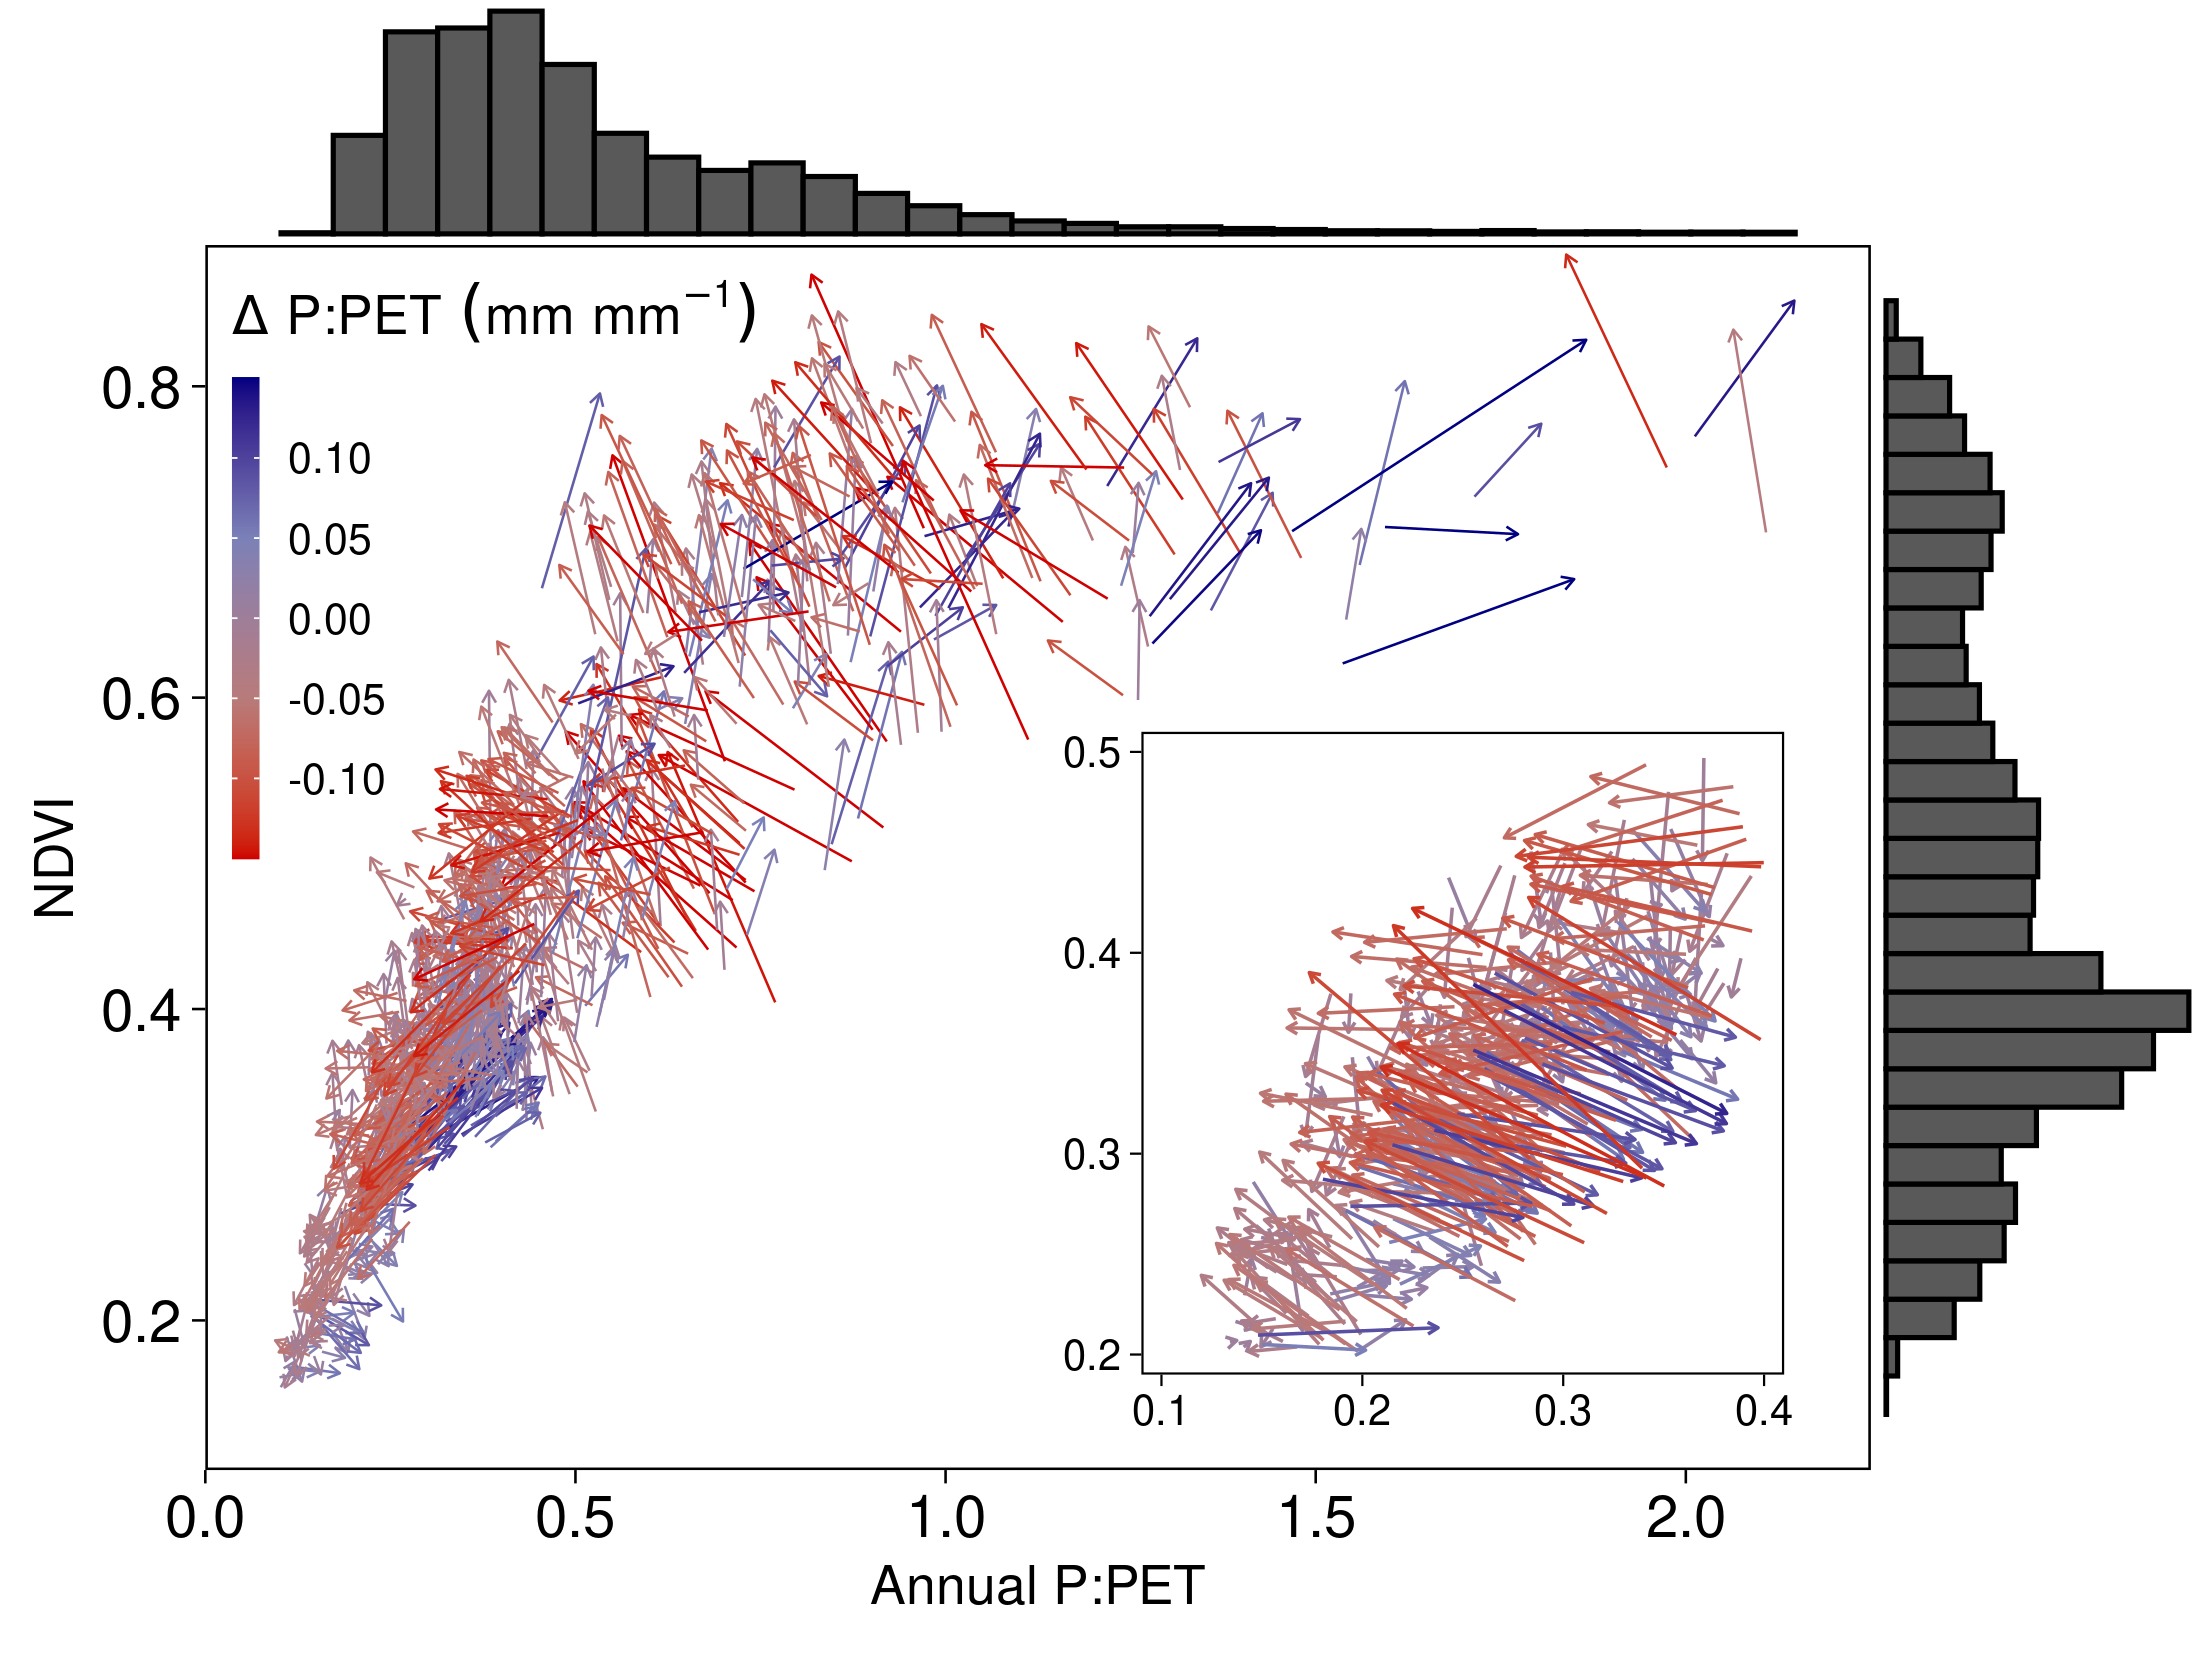
\includegraphics[width=16cm]{../../figures/Fig1_ndvi_ppet_vectorPlot_wInset} \caption{Individual grid cell temporal 38-year trajectories of the normalized difference vegetation index (NDVI) and the ratio of annual precipitation (P) to potential evapotranspiration (PET). A vector field plot showing the direction of change in mean annual NDVI and P:PET between 1982-1986 and 2015-2019 for 1000 randomly sampled grid-cell locations (color indicates direction of change in P:PET as indicated by legend). An inset shows a magnification of the samples from the 0.1-0.4 P:PET range. The distributions of mean P:PET ($mm\,mm^{-1}$) and NDVI for the period of 1982-1986 are shown as histograms above and to the right of the main panel. Note that the majority of arrows shift towards higher aridity (lower P:PET) and higher NDVI.}\label{fig:fig.align:"left"}
\end{figure}
\clearpage
\begin{figure}
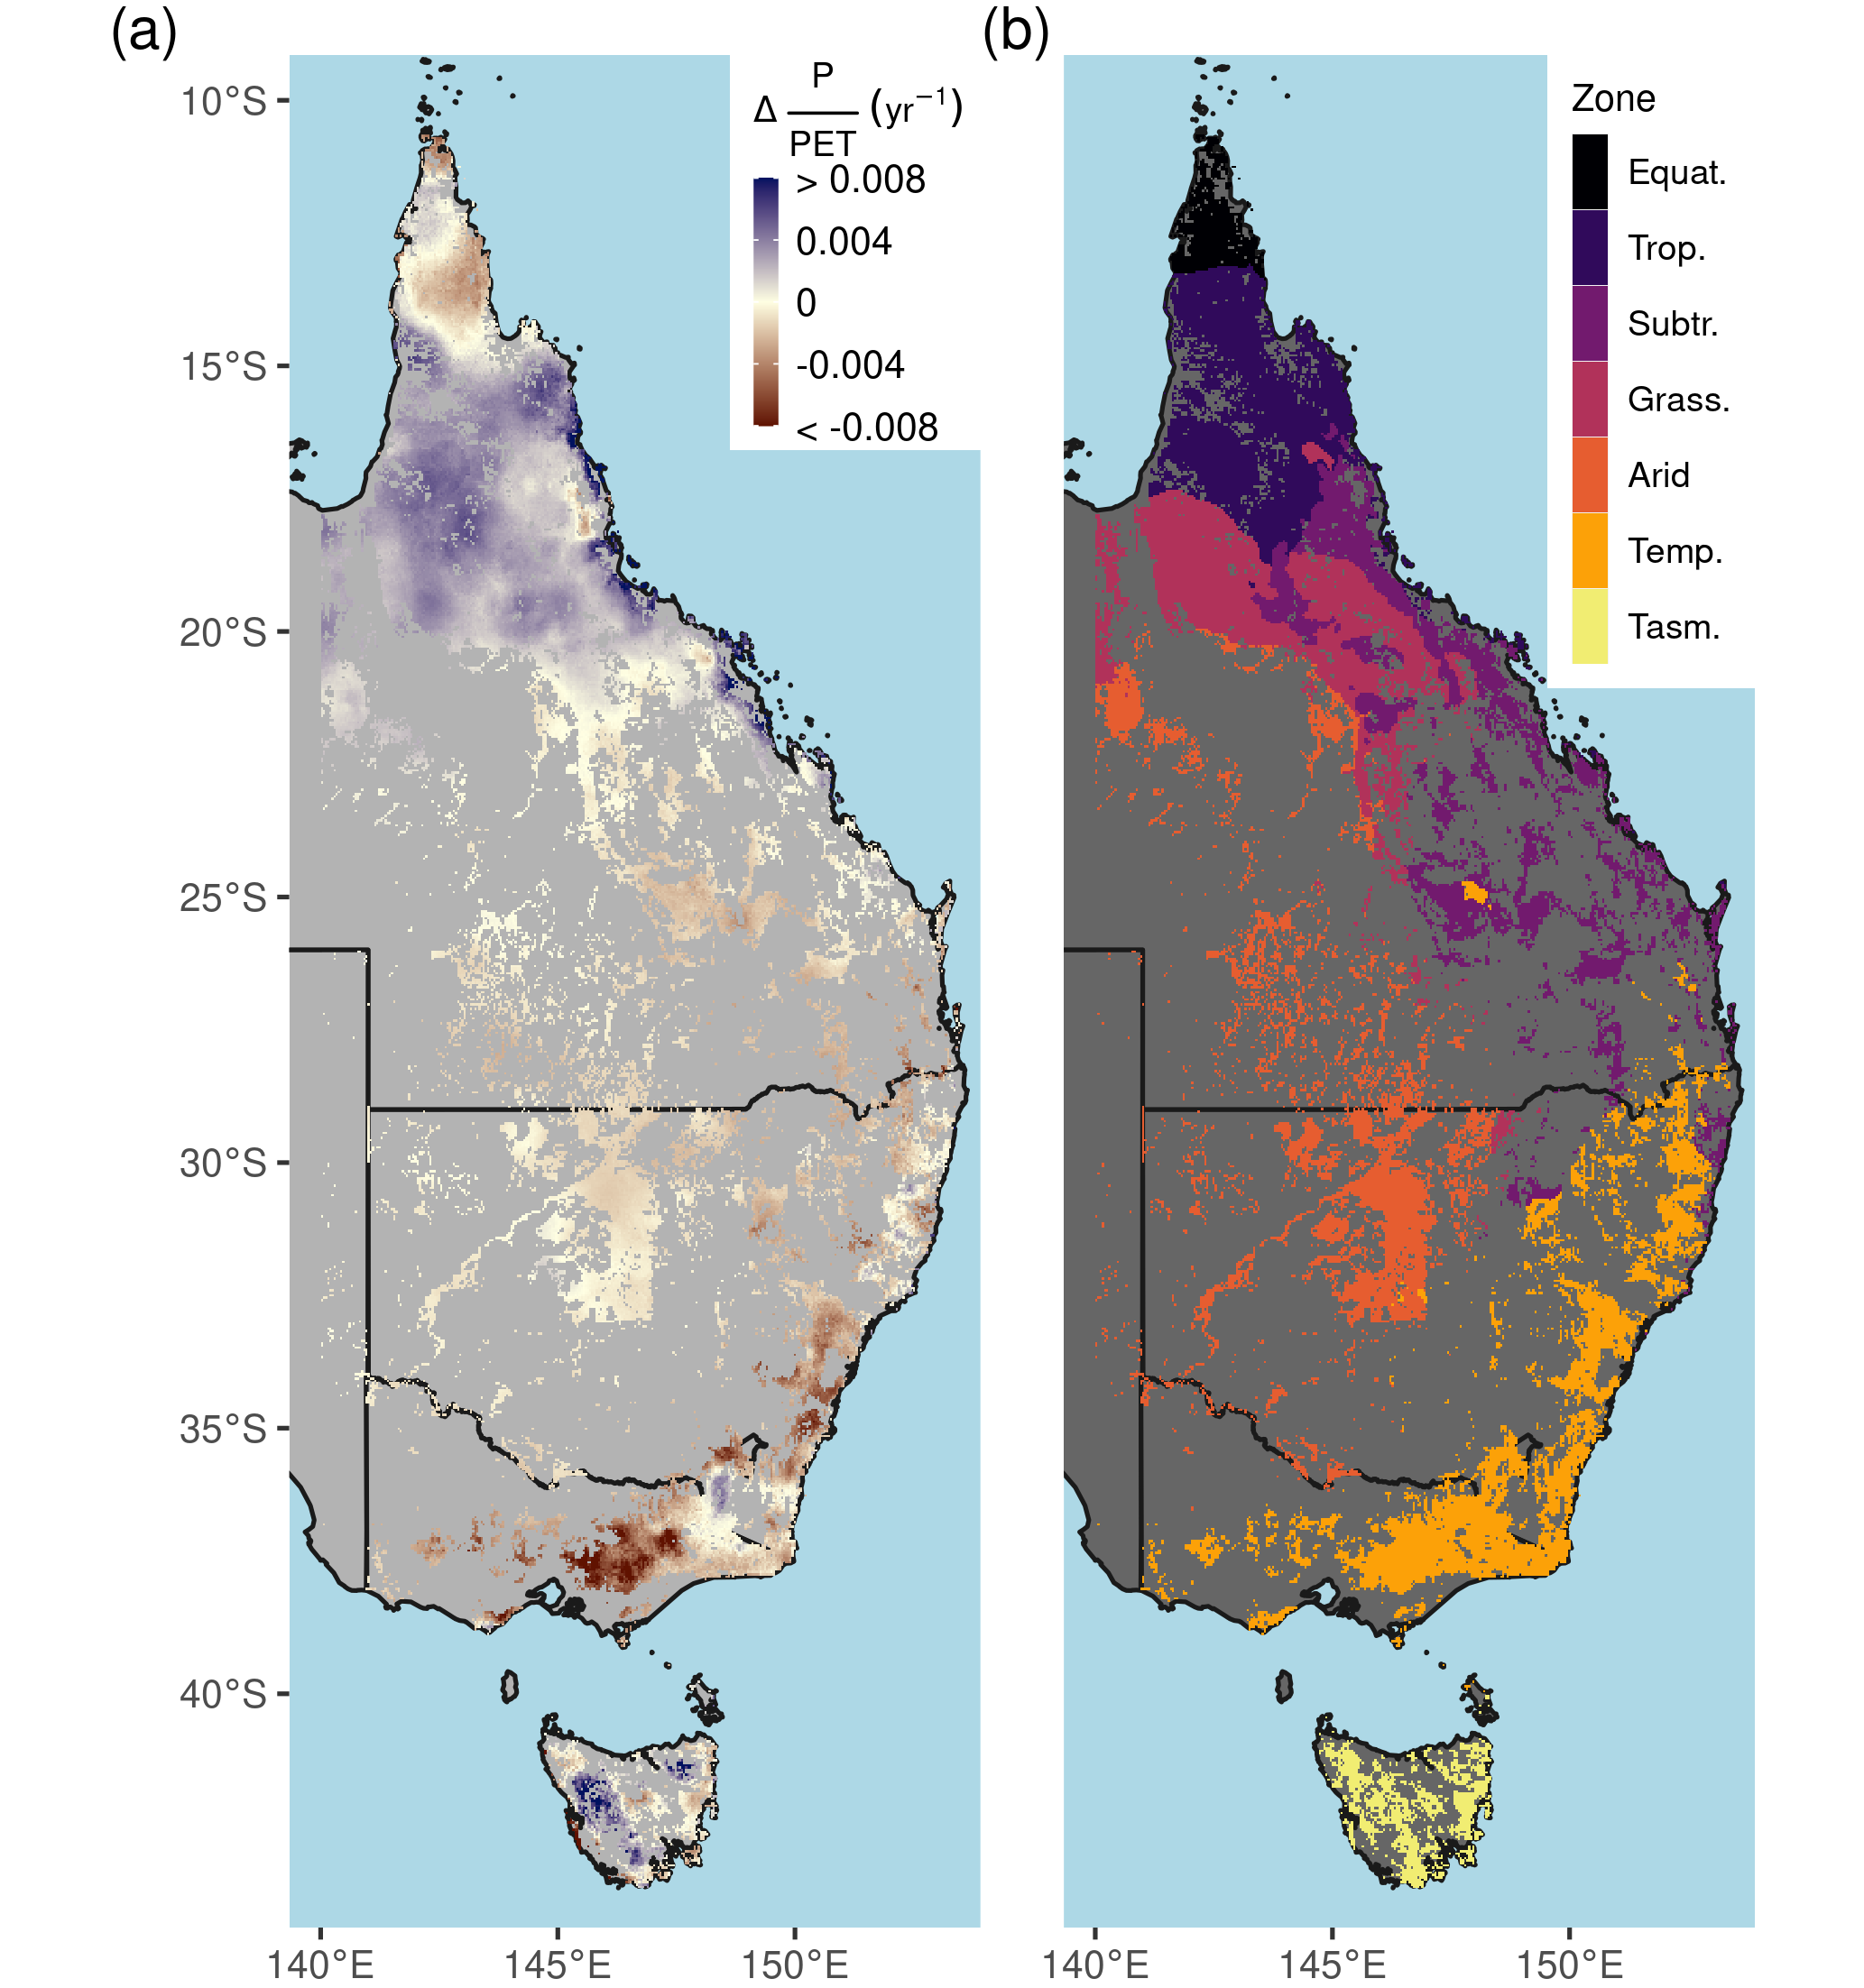
\includegraphics[width=12cm]{../../figures/Fig2_PPET-TheilSen_map-Koppen} \caption{Long-term aridity change and climate zones. (a) The linear trend of annual P:PET (the moisture index) between 1982-2019, (b) Simplified Köppen climate zones. Climate zone abbreviations correspond to Equatorial (Equat.), Tropical (Trop.), Subtropical (Subtr.), Grassland (Grass.), Temperate (Temp.), and Temperate Tasmania (Tasm.).}\label{fig:unnamed-chunk-1}
\end{figure}
\clearpage

\section{Results}

\subsection{Long-term Greening in a changing climate}

Parts of northern Queensland grew wetter, but aridity (as measured by
reduced P:PET; the moisture index, MI) in over 52\% of eastern
Australian woody ecosystems since 1982 (Figs. 1,2a). Aridity decreased
over northern Queensland encompassing the entirety of Equatorial and
Tropical regions, and most of the Grassland and Subtropical regions,
driven by large wet-season increases in precipitation (Fig S2a).
Widespread increases in PET were evident from September-February (Fig
S2b). At the same time as these changes in climate were occurring, over
92\% of these regions experienced overall greening (Fig. 3a), including
regions where P:PET declined (Figs. 1,2b,S3). The relative increases in
NDVI were comparable between the earlier AVHRR epoch (1982-2000) and the
later MODIS epoch (2001-2019) at 5.7\% (CI={[}-2.9\%, +20.3\%{]}) and
5.1\% (CI={[}-6.4\%, +20.1\%{]}), respectively. However, the spatial
patterns of greening/browning differed between epochs (Fig. 3b), and
most regions also showed high decadal-scale variability of
greening/browning trends (Fig. 4). The overall greening trends between
the AVHRR 1982-2000 epoch and the MODIS 2001-2019 epoch generally agree
across regions and seasons. However linear NDVI trends fit over shorter
intervals of 10 years are much less consistent (Fig. 4), exemplifying
the importance of estimating trends over long enough periods to average
over decadal-scale variability. Long term browning only occurred in the
Arid region (Fig. 3,4). Nevertheless, by examining NDVI trends over
nearly forty years, we were able to separate regional decadal-scale
variability from the overall, broad greening trend across eastern
Australia (Figs. 3,4,S3).

\clearpage
\begin{figure}
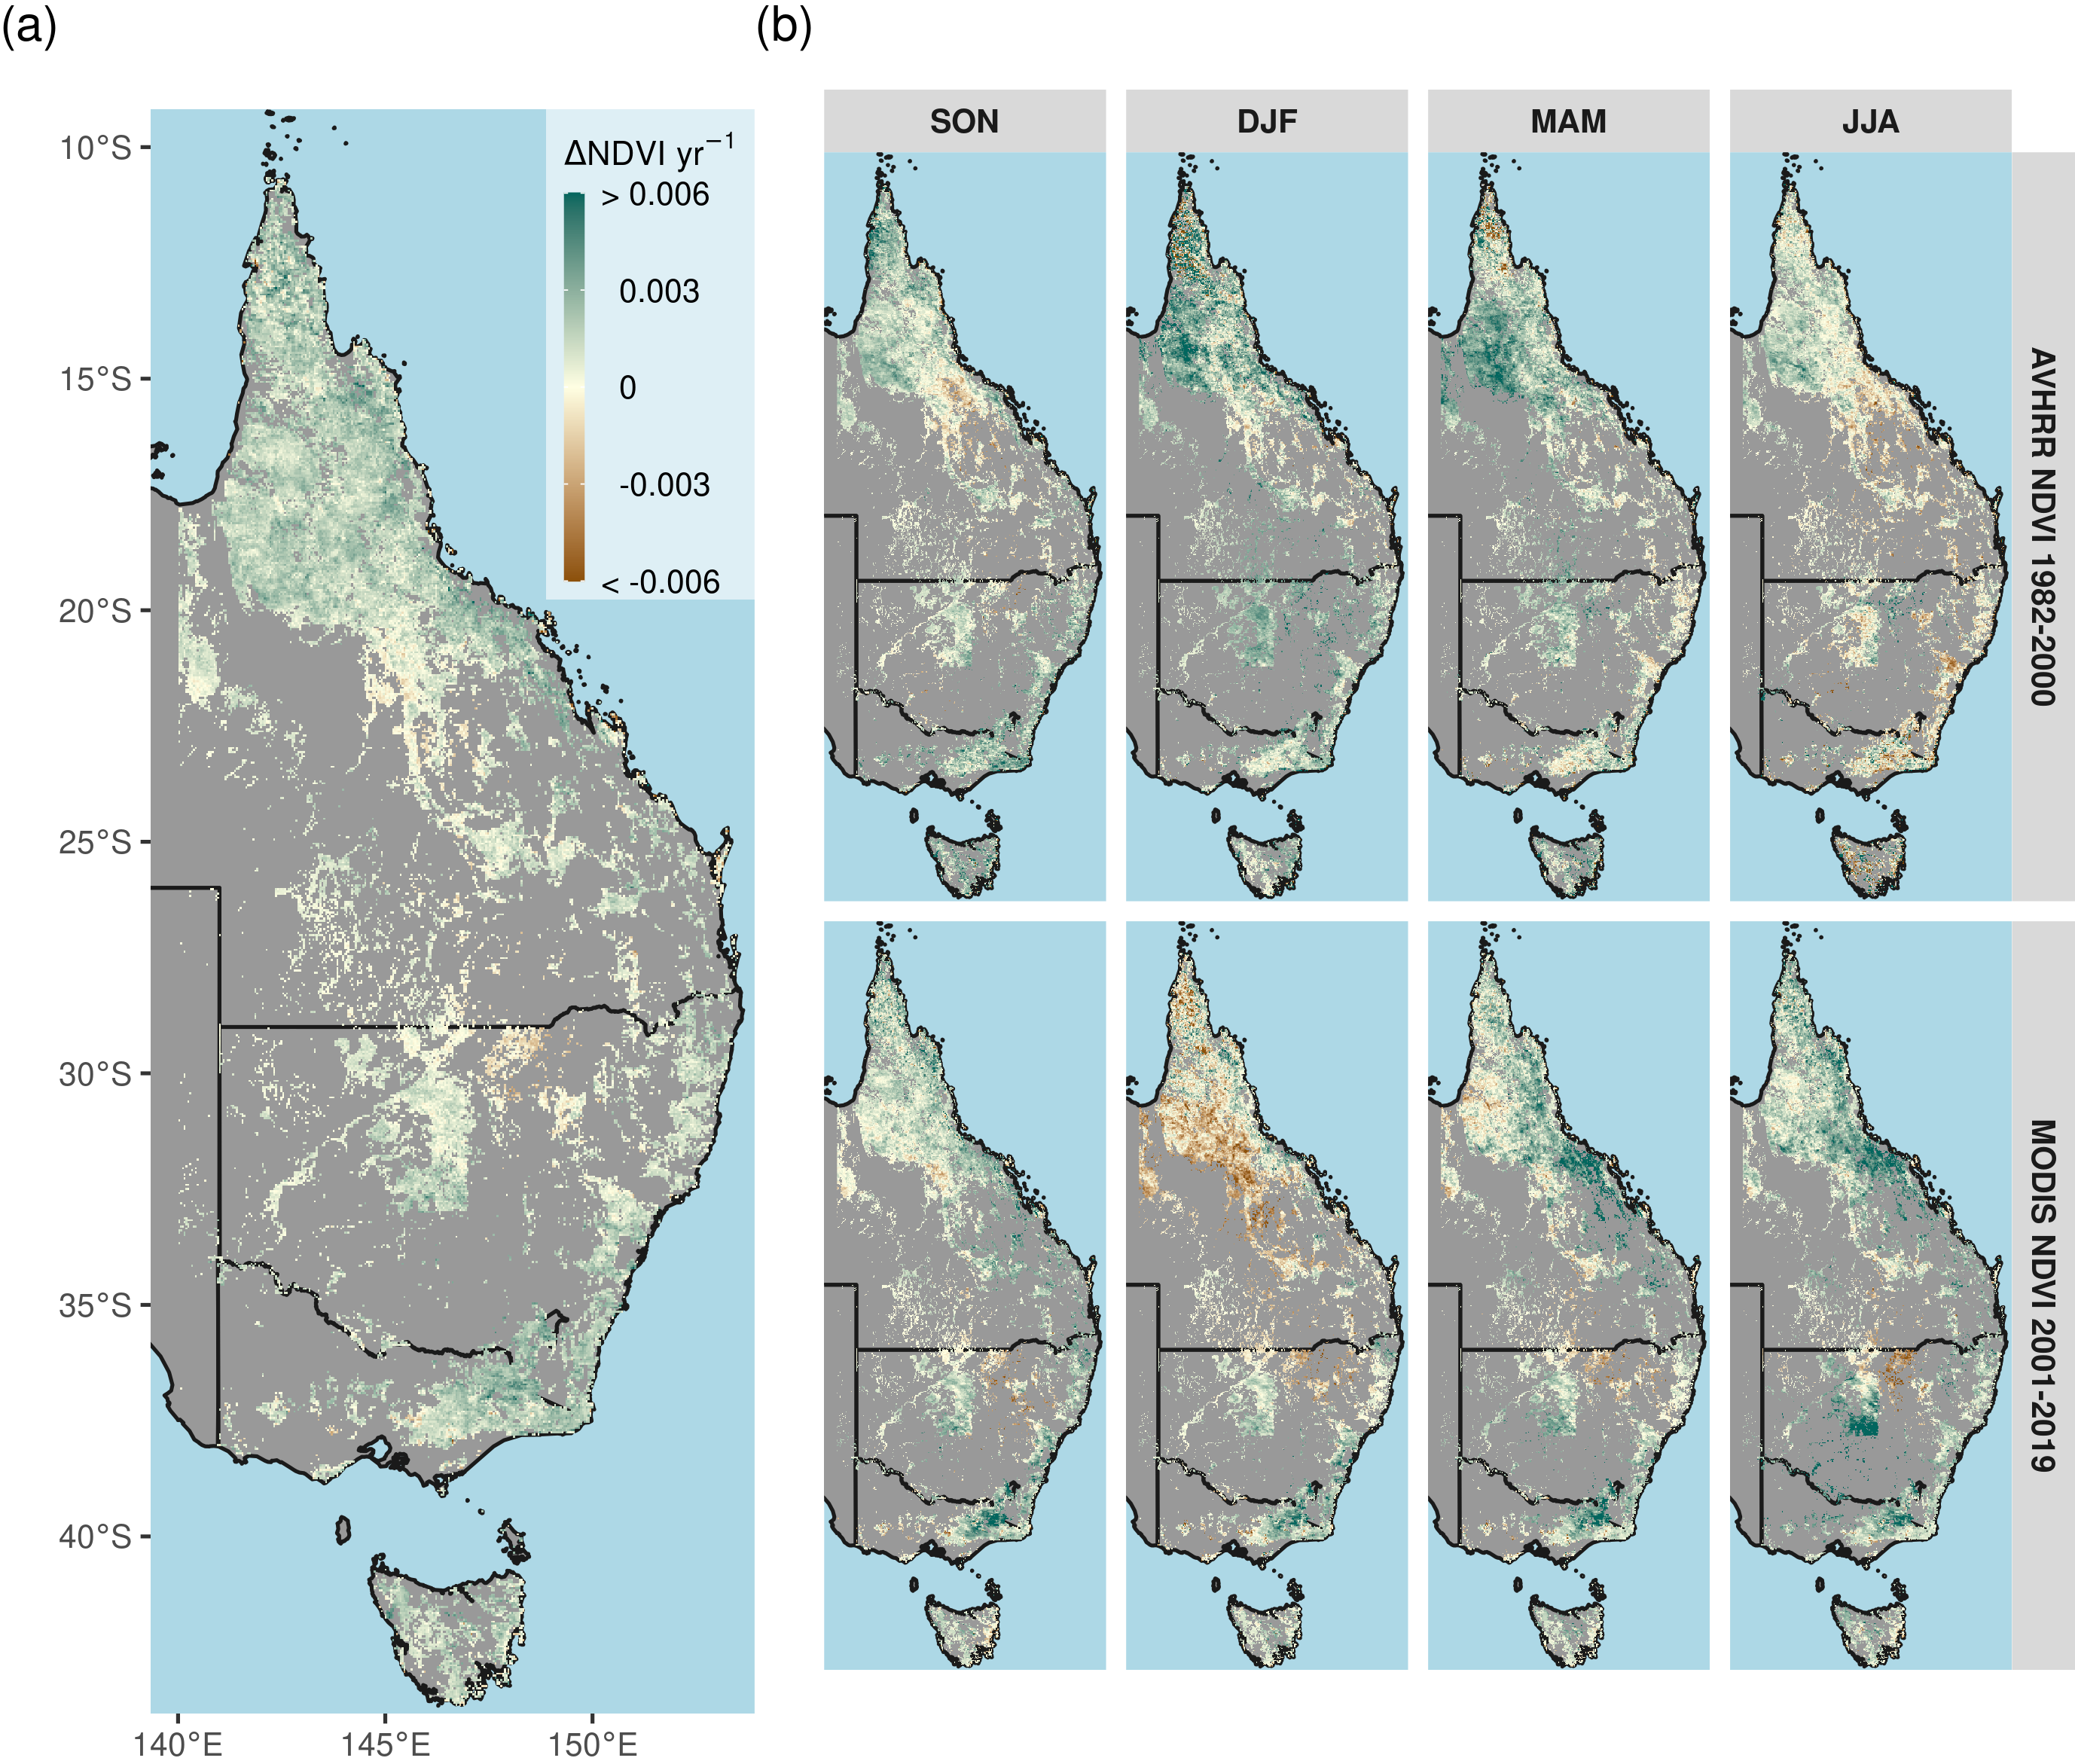
\includegraphics[width=12cm]{../../figures/Fig3_ndvi-annual-rlm_ndvi-seasonal-TheilSen-trend-by-epoch} \caption{Overall long-term NDVI change and change shown by satellite epoch and season. (a) The annual rate of NDVI change from the merged satellite record spanning 1982-2019. The seasonal AVHRR NDVI between 1982-2000 (b-top) and MODIS NDVI between 2001-2019 (b-bottom). Non woody ecosystem regions are masked in gray. A notable browning trend is evident at the interface of the Grassland and Arid regions during DJF of the MODIS time period.\linebreak Note: Season abbreviations correspond to September-October (SON), December-February (DJF), March-May (MAM), and July-August (JJA).}\label{fig:unnamed-chunk-2}
\end{figure}
\clearpage

\begin{figure}
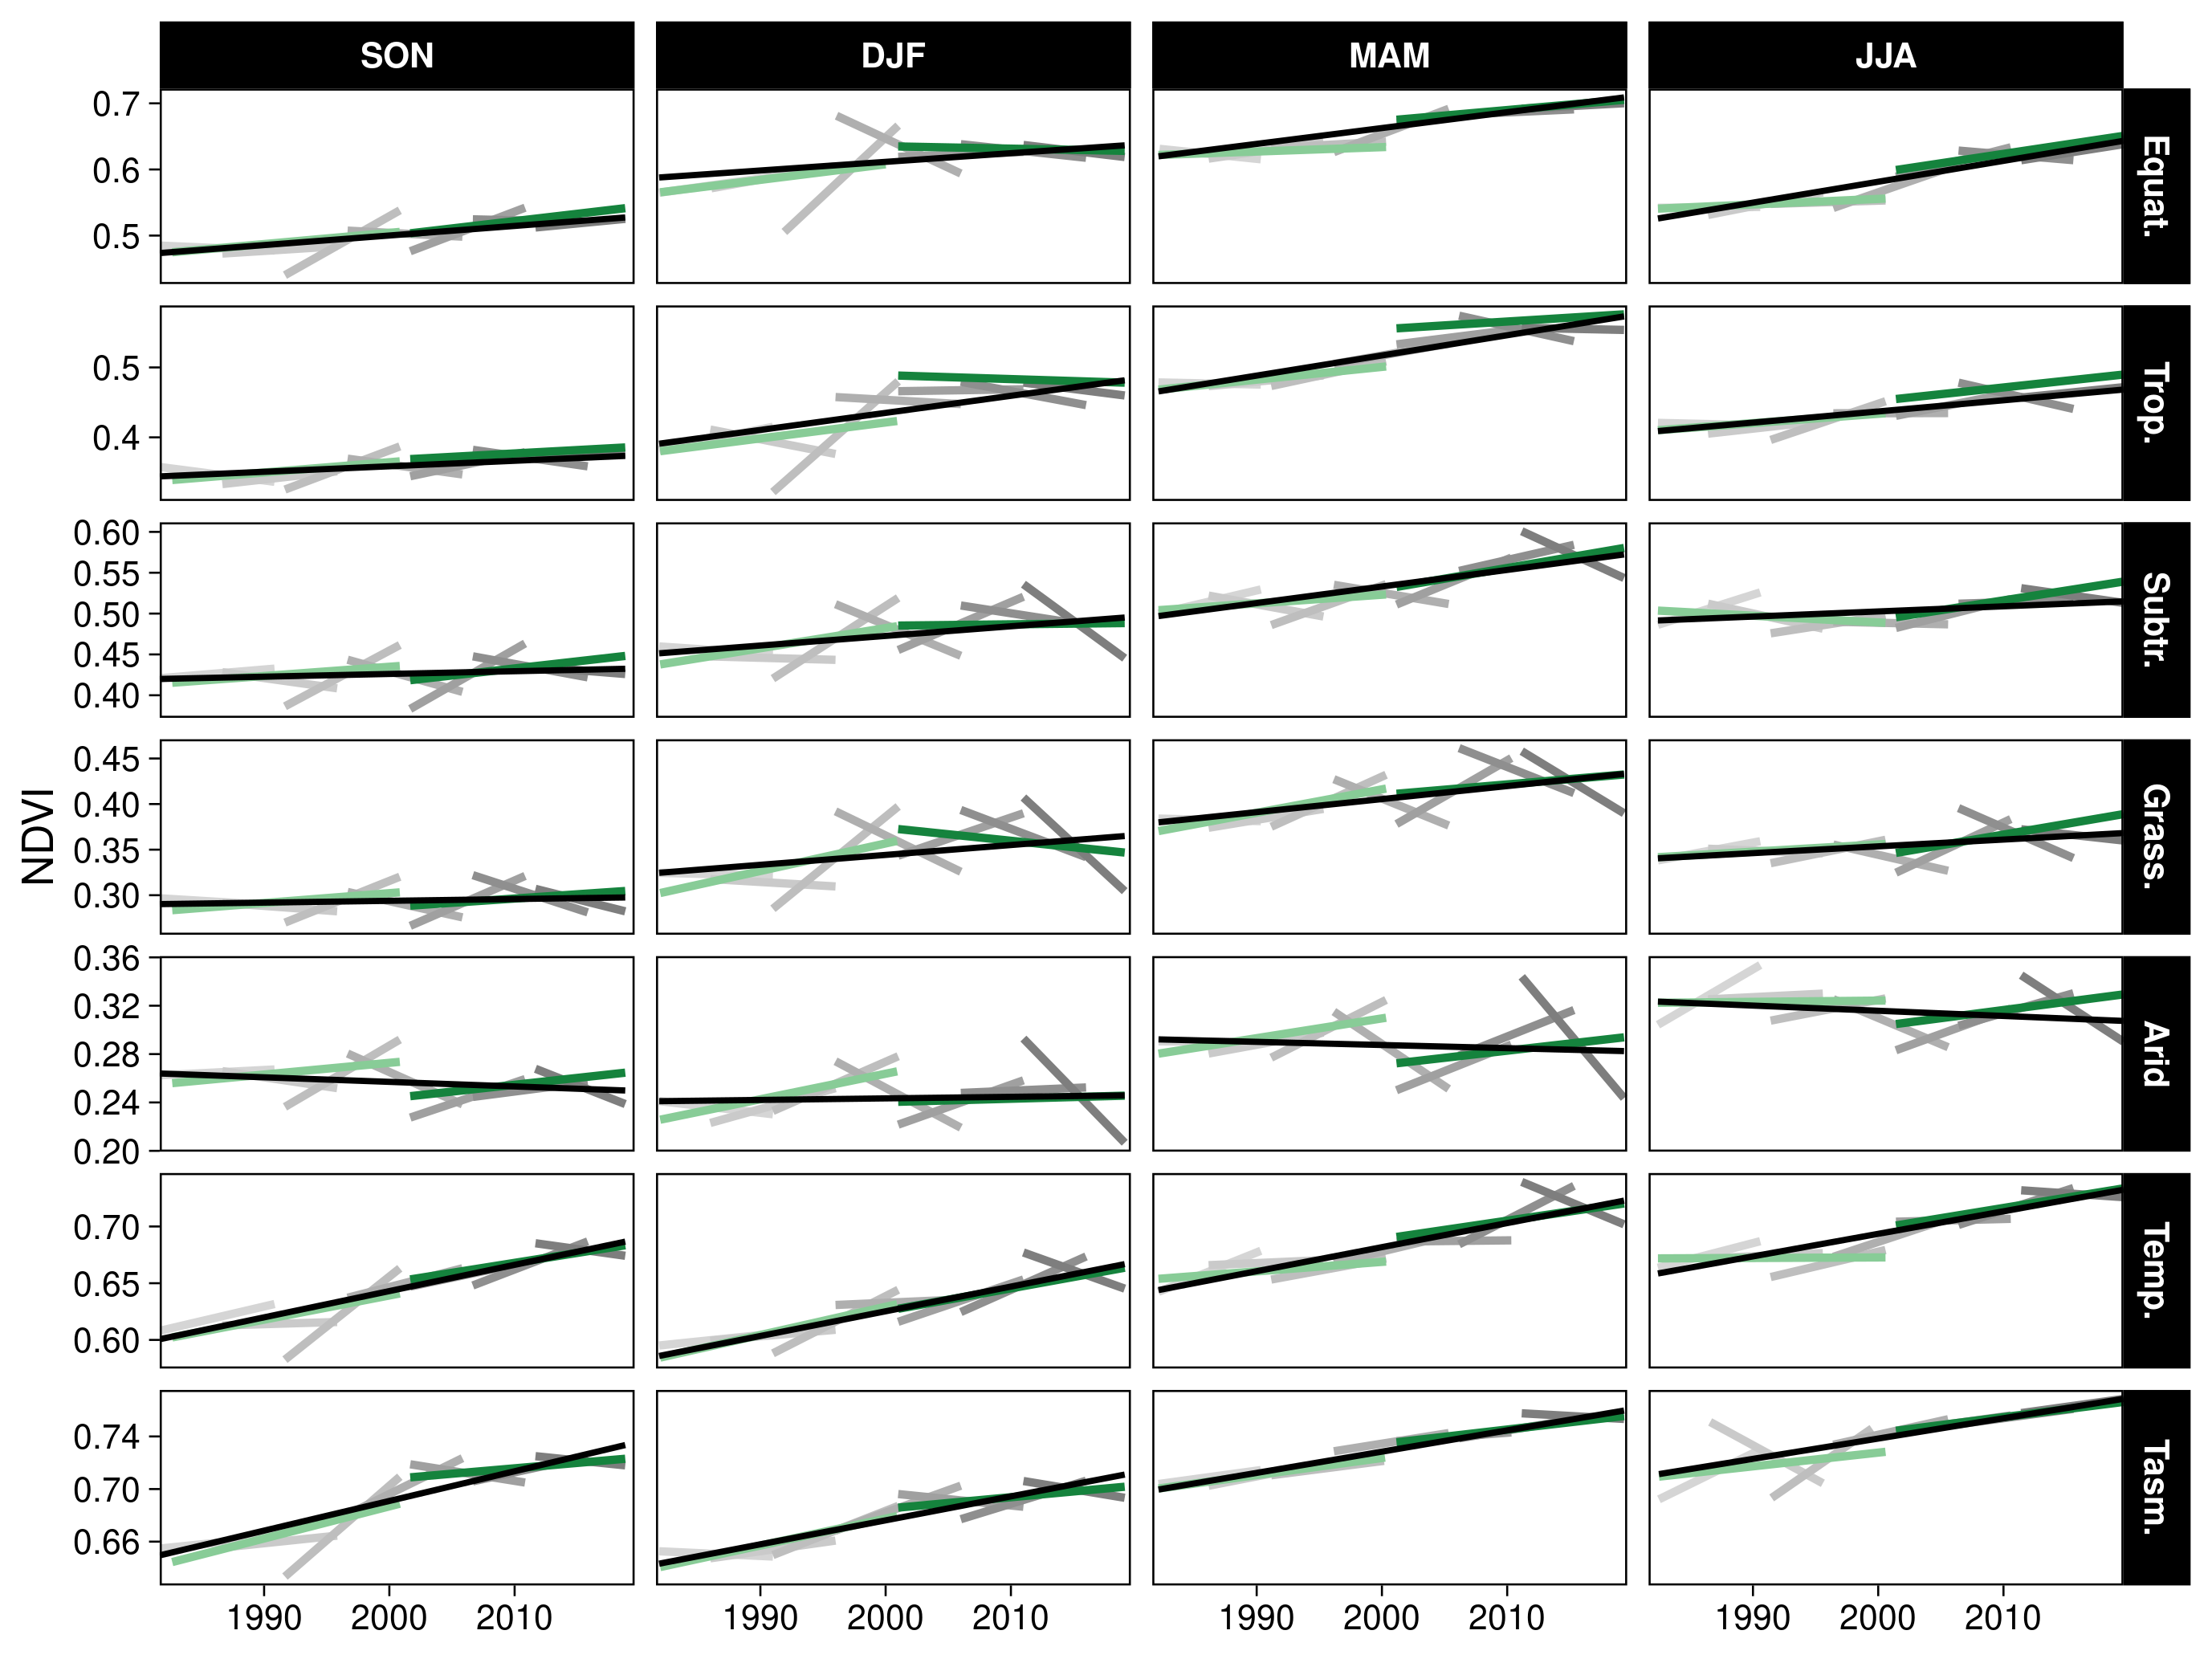
\includegraphics[width=12cm]{../../figures/Fig4_ndvi_lin_rlm_trend_10yr_segs_by_Koppen} \caption{Variability of linear trends over varying time periods by season and climate zone. The (black) line represents the overall 1982-2019 trend, the (light green) line represents the calibrated AVHRR 1982-2000, and the (green) line represents the MODIS 2001-2019. Gray colors indicate linear trends from overlapping 10 year time intervals. The boundaries of the climate zones are shown in Figure 7. \linebreak Note: Climate zone abbreviations correspond to Equatorial (Equat.), Tropical (Trop.), Subtropical (Subtr.), Grassland (Grass.), Temperate (Temp.), and Temperate Tasmania (Tasm.). Season abbreviations correspond to September-October (SON), December-February (DJF), March-May (MAM), and July-August (JJA).}\label{fig:unnamed-chunk-3}
\end{figure}
\clearpage

\subsection{\texorpdfstring{Empirical attribution of the
CO\textsubscript{2} effect}{Empirical attribution of the CO2 effect}}

We found consistently positive NDVI responses to CO\textsubscript{2}
across the moisture gradient of P:PET for all seasons, with the greatest
increases located in regions of higher P:PET (\textgreater0.5) (Fig. 5).
The nonlinear Weibull models showed a larger CO\textsubscript{2}
attributable effect on NDVI in regions of higher P:PET (Fig. 5), but the
effect size of the NDVI response to CO\textsubscript{2} was largely
consistent across model forms (Figs. S4-7). The
CO\textsubscript{2}-attributable increase in NDVI between 1982-2019
ranged from approximately 5\% in the Arid interior regions to
\textgreater20\% in the wettest Tropical and Temperate regions (Fig.
5a). This was consistent with linear model forms when fit for individual
grid cell locations (equation 8; Fig. 6), as well as by comparing the
CO\textsubscript{2} effect size across 16 linear models fit for grid
cell locations grouped into bins spanning 0.1 increments of P:PET
(equation 7; Fig. S4). The GAM fit across grid cell locations also
indicated a larger CO\textsubscript{2} effect in regions with higher
P:PET (Figs. 6,7b). Quantile regression with generalized additive models
showed a pronounced response to CO\textsubscript{2} across the
distribution of pixels with both low and high NDVI (10 - 97.5
percentiles) across the full aridity gradient of P:PET (Fig. S7).

\clearpage
\begin{figure}
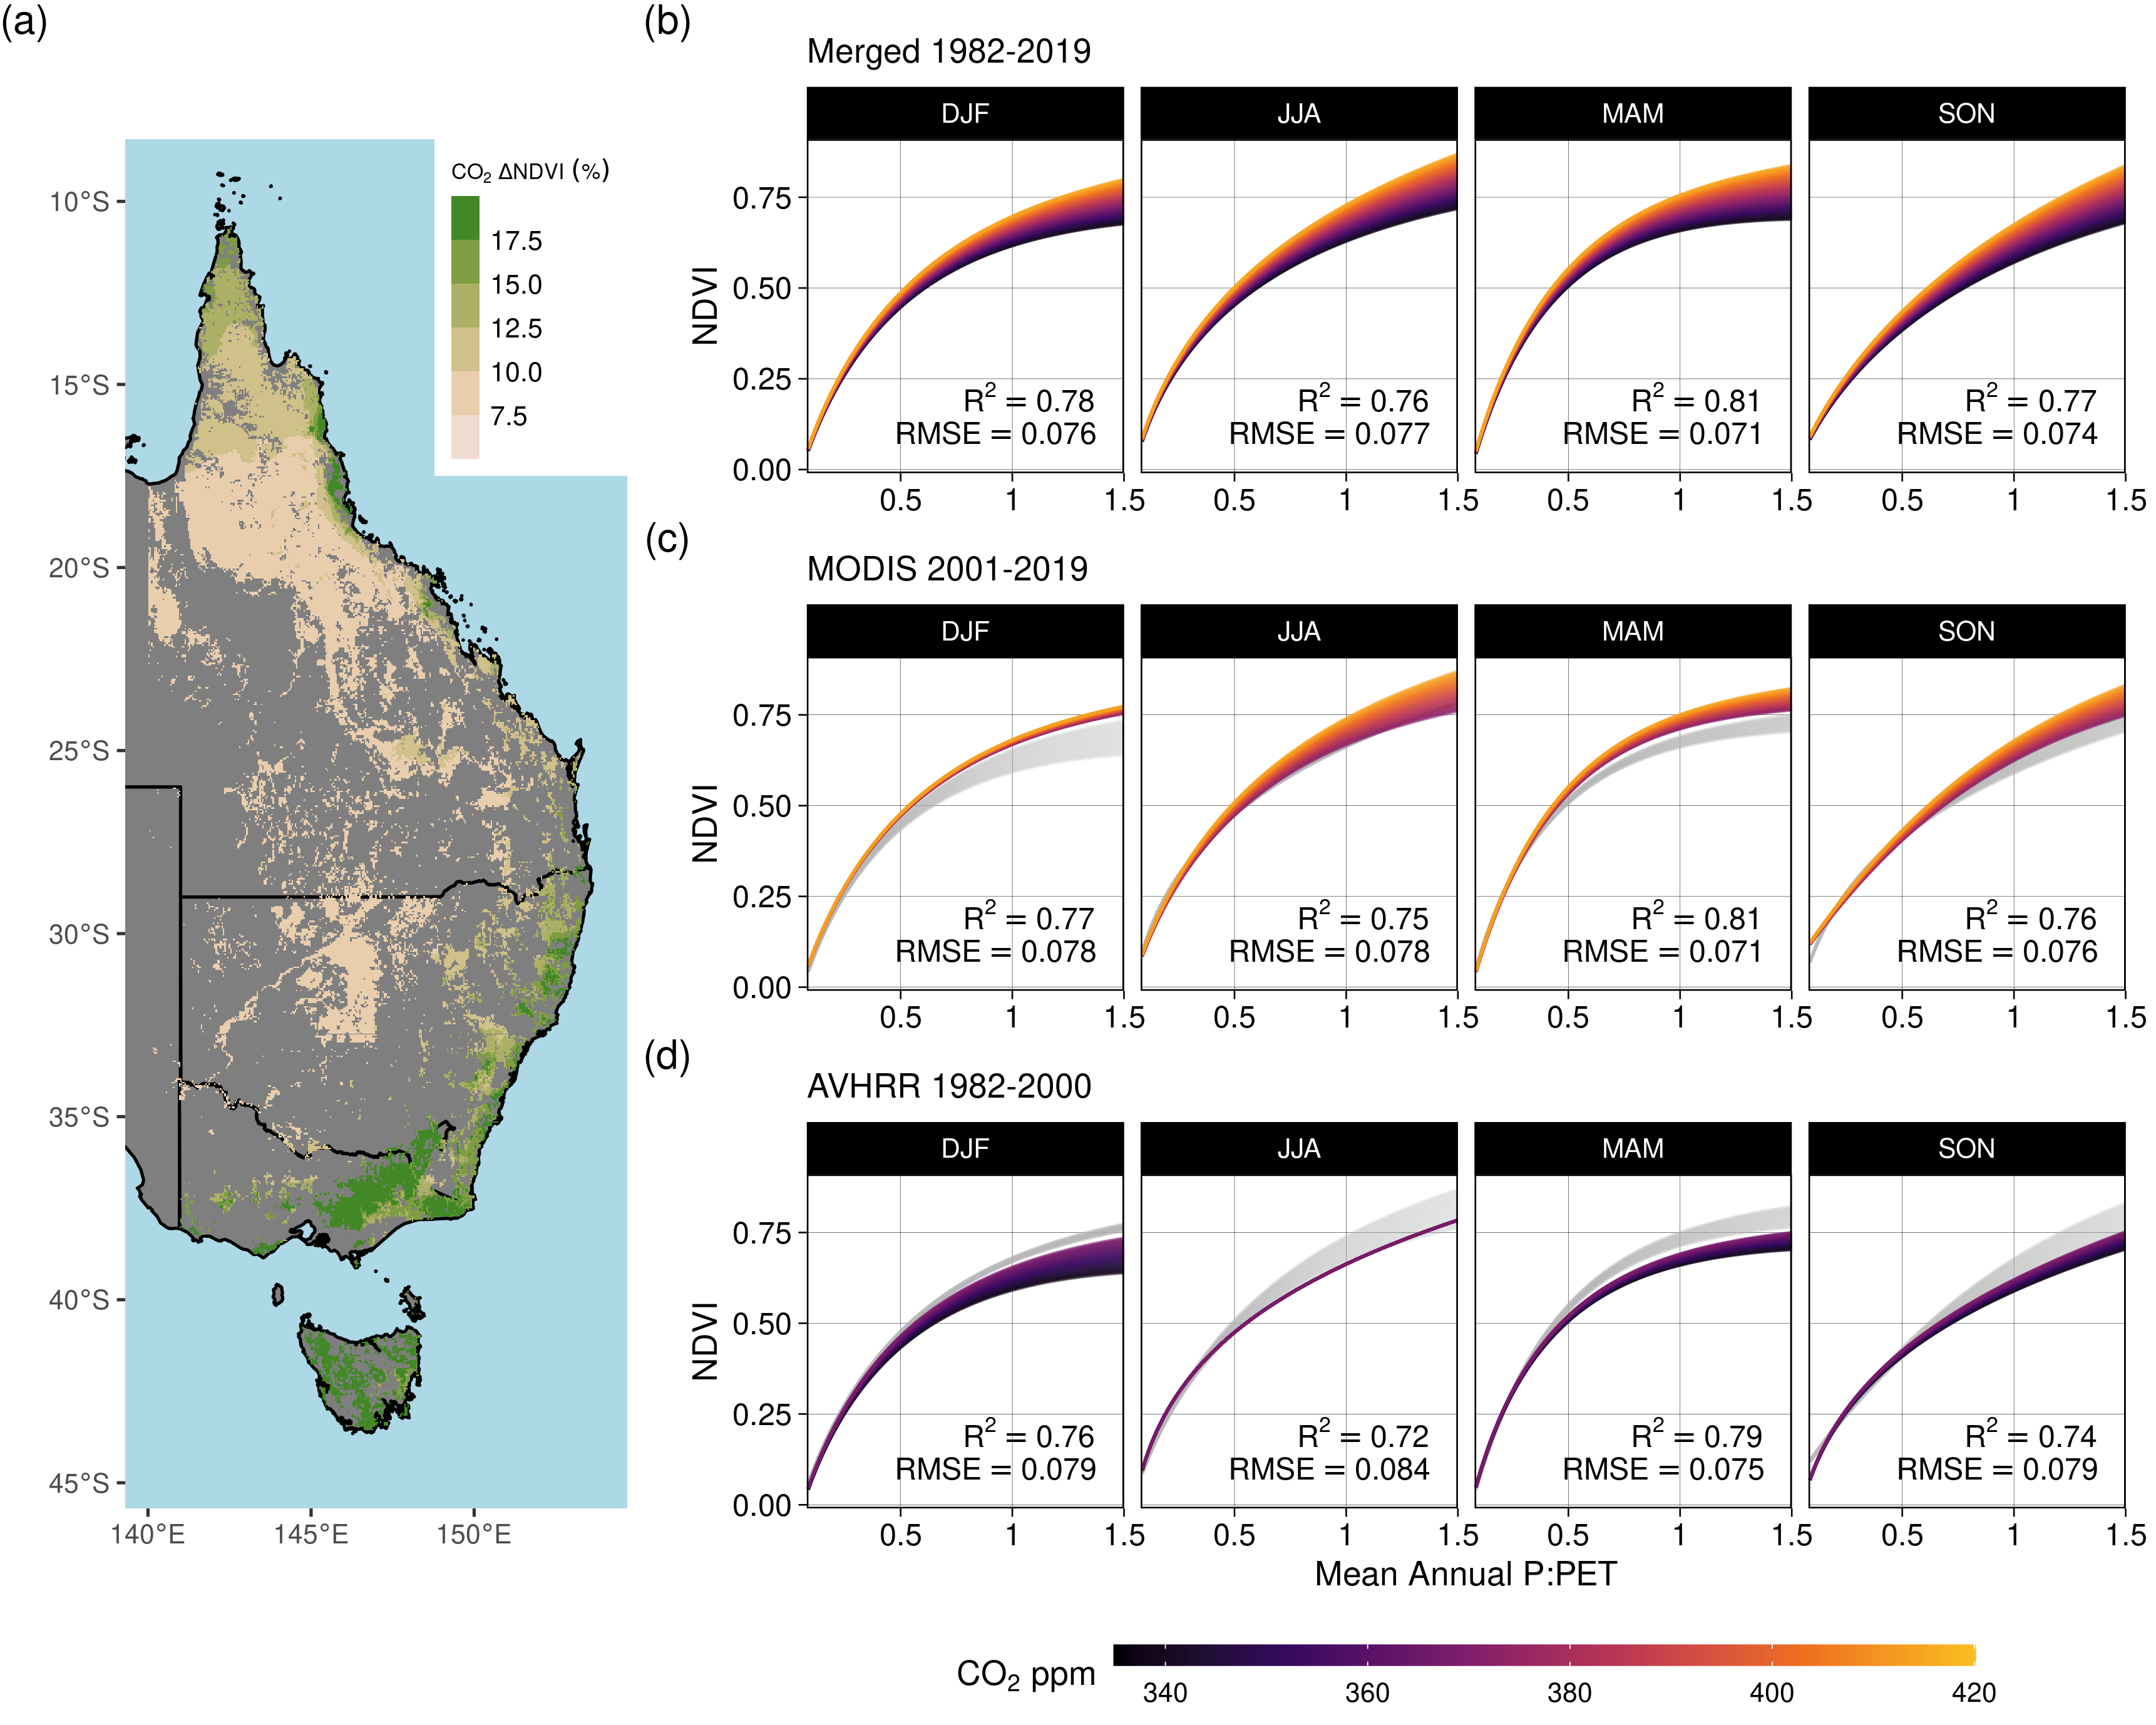
\includegraphics[width=12cm]{../../figures/Fig5_n4_ndvi_map_weibull_ppet_x_co2_modeled_effect} \caption{Effect of increasing $CO_2$ on seasonal NDVI across P:PET. Predictions of seasonal NDVI as a function of mean annual P:PET fit using a standard Weibull function (methods - eq 2), modified with linear effects of $CO_2$, the running 12-month anomaly of P:PET, and the satellite sensor. The $CO_2$ concentration gradient represents the atmospheric $CO_2$ change between 1982-2019. Panel (a) maps the total predicted contribution of $CO_2$ towards the relative increase of NDVI between 1982-2019 assuming no anomaly of P:PET. Panel (b) shows the merged sensor response between 1982-2019 across the gradient of P:PET, (c) shows the model response when fit using just MODIS MCD43 data between 2001-2019, and (d) shows the response when the model was fit with the recalibrated AVHRR data between 1982-2000. The AVHRR and MODIS satellite epoch NDVI predictions are plotted in gray for panels B and C, respectively.}\label{fig:unnamed-chunk-4}
\end{figure}
\clearpage

A recent study found the global CO\textsubscript{2} fertilization effect
was halved between the 1980s and 2000s
\citep{wangRecentGlobalDecline2020}. In contrast to the estimates over
eastern Australia from wangRecentGlobalDecline2020 over, we found no
consistent evidence of a decline in the effect of CO\textsubscript{2} on
NDVI through time. Neither the GAM estimates nor the robust linear model
estimates of the CO\textsubscript{2} effect showed any consistent
evidence of a weakening CO\textsubscript{2} effect between 1982-2000 and
2001-2019 (Fig. 6). The central 25-75\% percentiles of the distribution
of robust linear model effect sizes overlapped in all regions between
epochs. The central 25-75\% of the GAM estimated distributions also
overlapped, with the exception of the Grassland and Arid regions where
the CO\textsubscript{2} effect was larger during 2001-2019. Consistent
with the finding of a greater CO\textsubscript{2} effect in wetter
regions (Fig. 5), the robust linear models and the GAM estimated the
CO\textsubscript{2} effect to be greatest in the Equatorial and Tropical
regions, and lowest in the Arid region (Fig. 6).

\clearpage
\begin{figure}
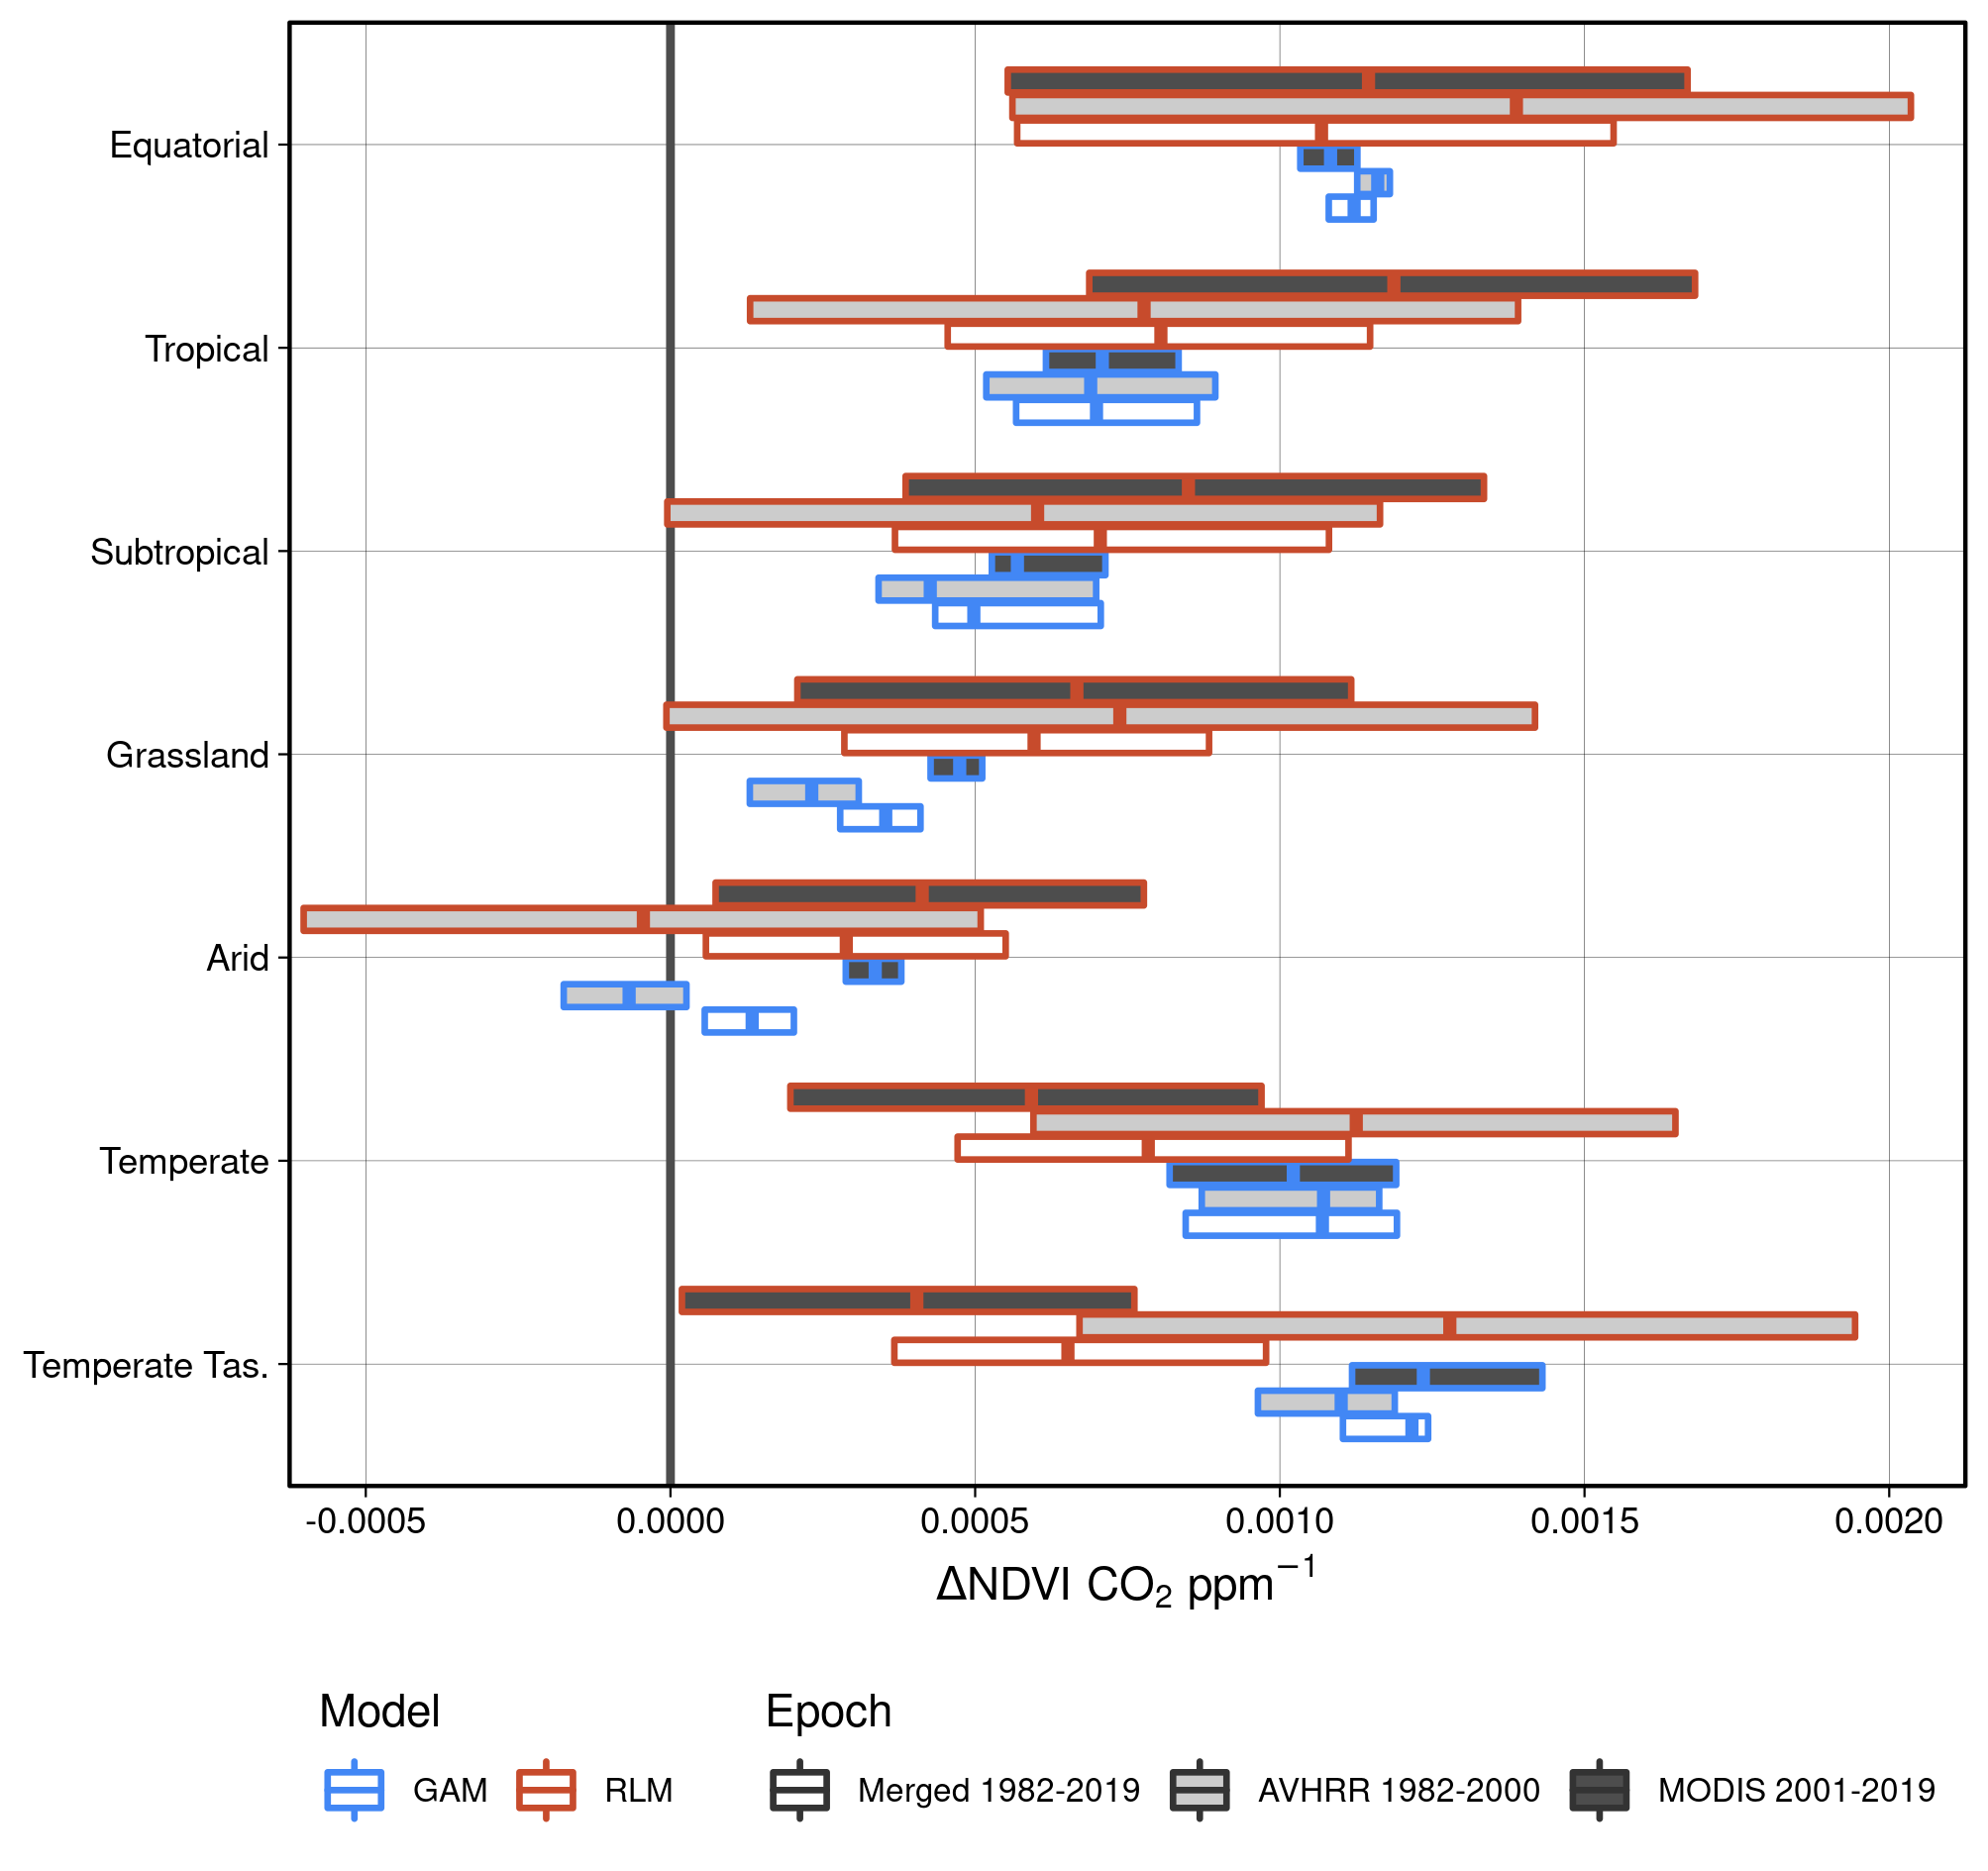
\includegraphics[width=14cm]{../../figures/Fig6_rlm_CO2_effect_by_epoch} \caption{Boxplot representation of the $CO_2$ attributable effect upon changing NDVI. Here the 25th, 50th, and 75th percentiles of the $CO_2$ attributable effect on NDVI are shown. The robust linear models (RLM; methods - eq 13) were fit for each individual grid cell location, whereas the generalized additive model (GAM; methods - eq 14) was fit using all grid cell locations. The distribution of RLMs yielded a median $R^2$ of 0.58 and RMSE of 0.025 over the merged period. The GAM had an overall $R^2$ of 0.91 and RMSE of 0.049.}\label{fig:unnamed-chunk-5}
\end{figure}
\clearpage

\subsection{\texorpdfstring{CO\textsubscript{2} driven greening and
expectations from water use
efficiency}{CO2 driven greening and expectations from water use efficiency}}

The range of statistically estimated CO\textsubscript{2}-attributable
greening responses was compared with the expectation from the
theoretical CO\textsubscript{2} water use efficiency model. The Donohue
et al.~(2013) CO\textsubscript{2} x WUE model (see methods) accounts for
changes in VPD, but assumes no change in water supply. Assuming an equal
split in the benefits of WUE between greater carbon assimilation and
increased foliage cover (see below for alternative assumptions), the
model predicted an 8.7\% (10-90\% percentile range {[}+6.8\%,+10.2\%{]})
increase in NDVI (proxy for foliage cover, see methods). This compared
to an estimated 11.7\% ({[}+4.6\%,+14.6\%{]}) relative increase from the
GAM, when accounting for simultaneous increase in VPD (which the WUE
accounts for), and factoring out the effects of changing precipitation
and PET (which the WUE model does not account for). We needed to assume
differing levels of allocation to foliar gain (i.e.~not 50\%) for the
theoretical WUE model to match the statistically estimated
CO\textsubscript{2} effect (Fig. 7d). Regions of higher P:PET
(Equatorial, Tropical, Temperate, and Temperate Tasmanian) required
greater allocation fractions than 50\%, whereas the allocation fraction
would be between 25-50\% for regions with lower P:PET (Arid, Grassland,
and Subtropical). In comparison, the PETA hypothesis
\citep{donohue_etal17} predicted the greatest CO\textsubscript{2} effect
on leaf area to be in regions with the lowest LAI, but this was not
supported by the statistically estimated CO\textsubscript{2} effect on
NDVI (Fig. S9). Despite having the lowest LAI, the Arid region received
the smallest CO\textsubscript{2} effect, but it is worth noting the Arid
region also experienced the greatest increase in VPD and reduction in P
over the 38 year period (Fig. 7a, S8). In contrast, the largest
estimated CO\textsubscript{2}-attributable effect on greening were found
to be in the Equatorial and Tropical areas.

\clearpage
\begin{figure}
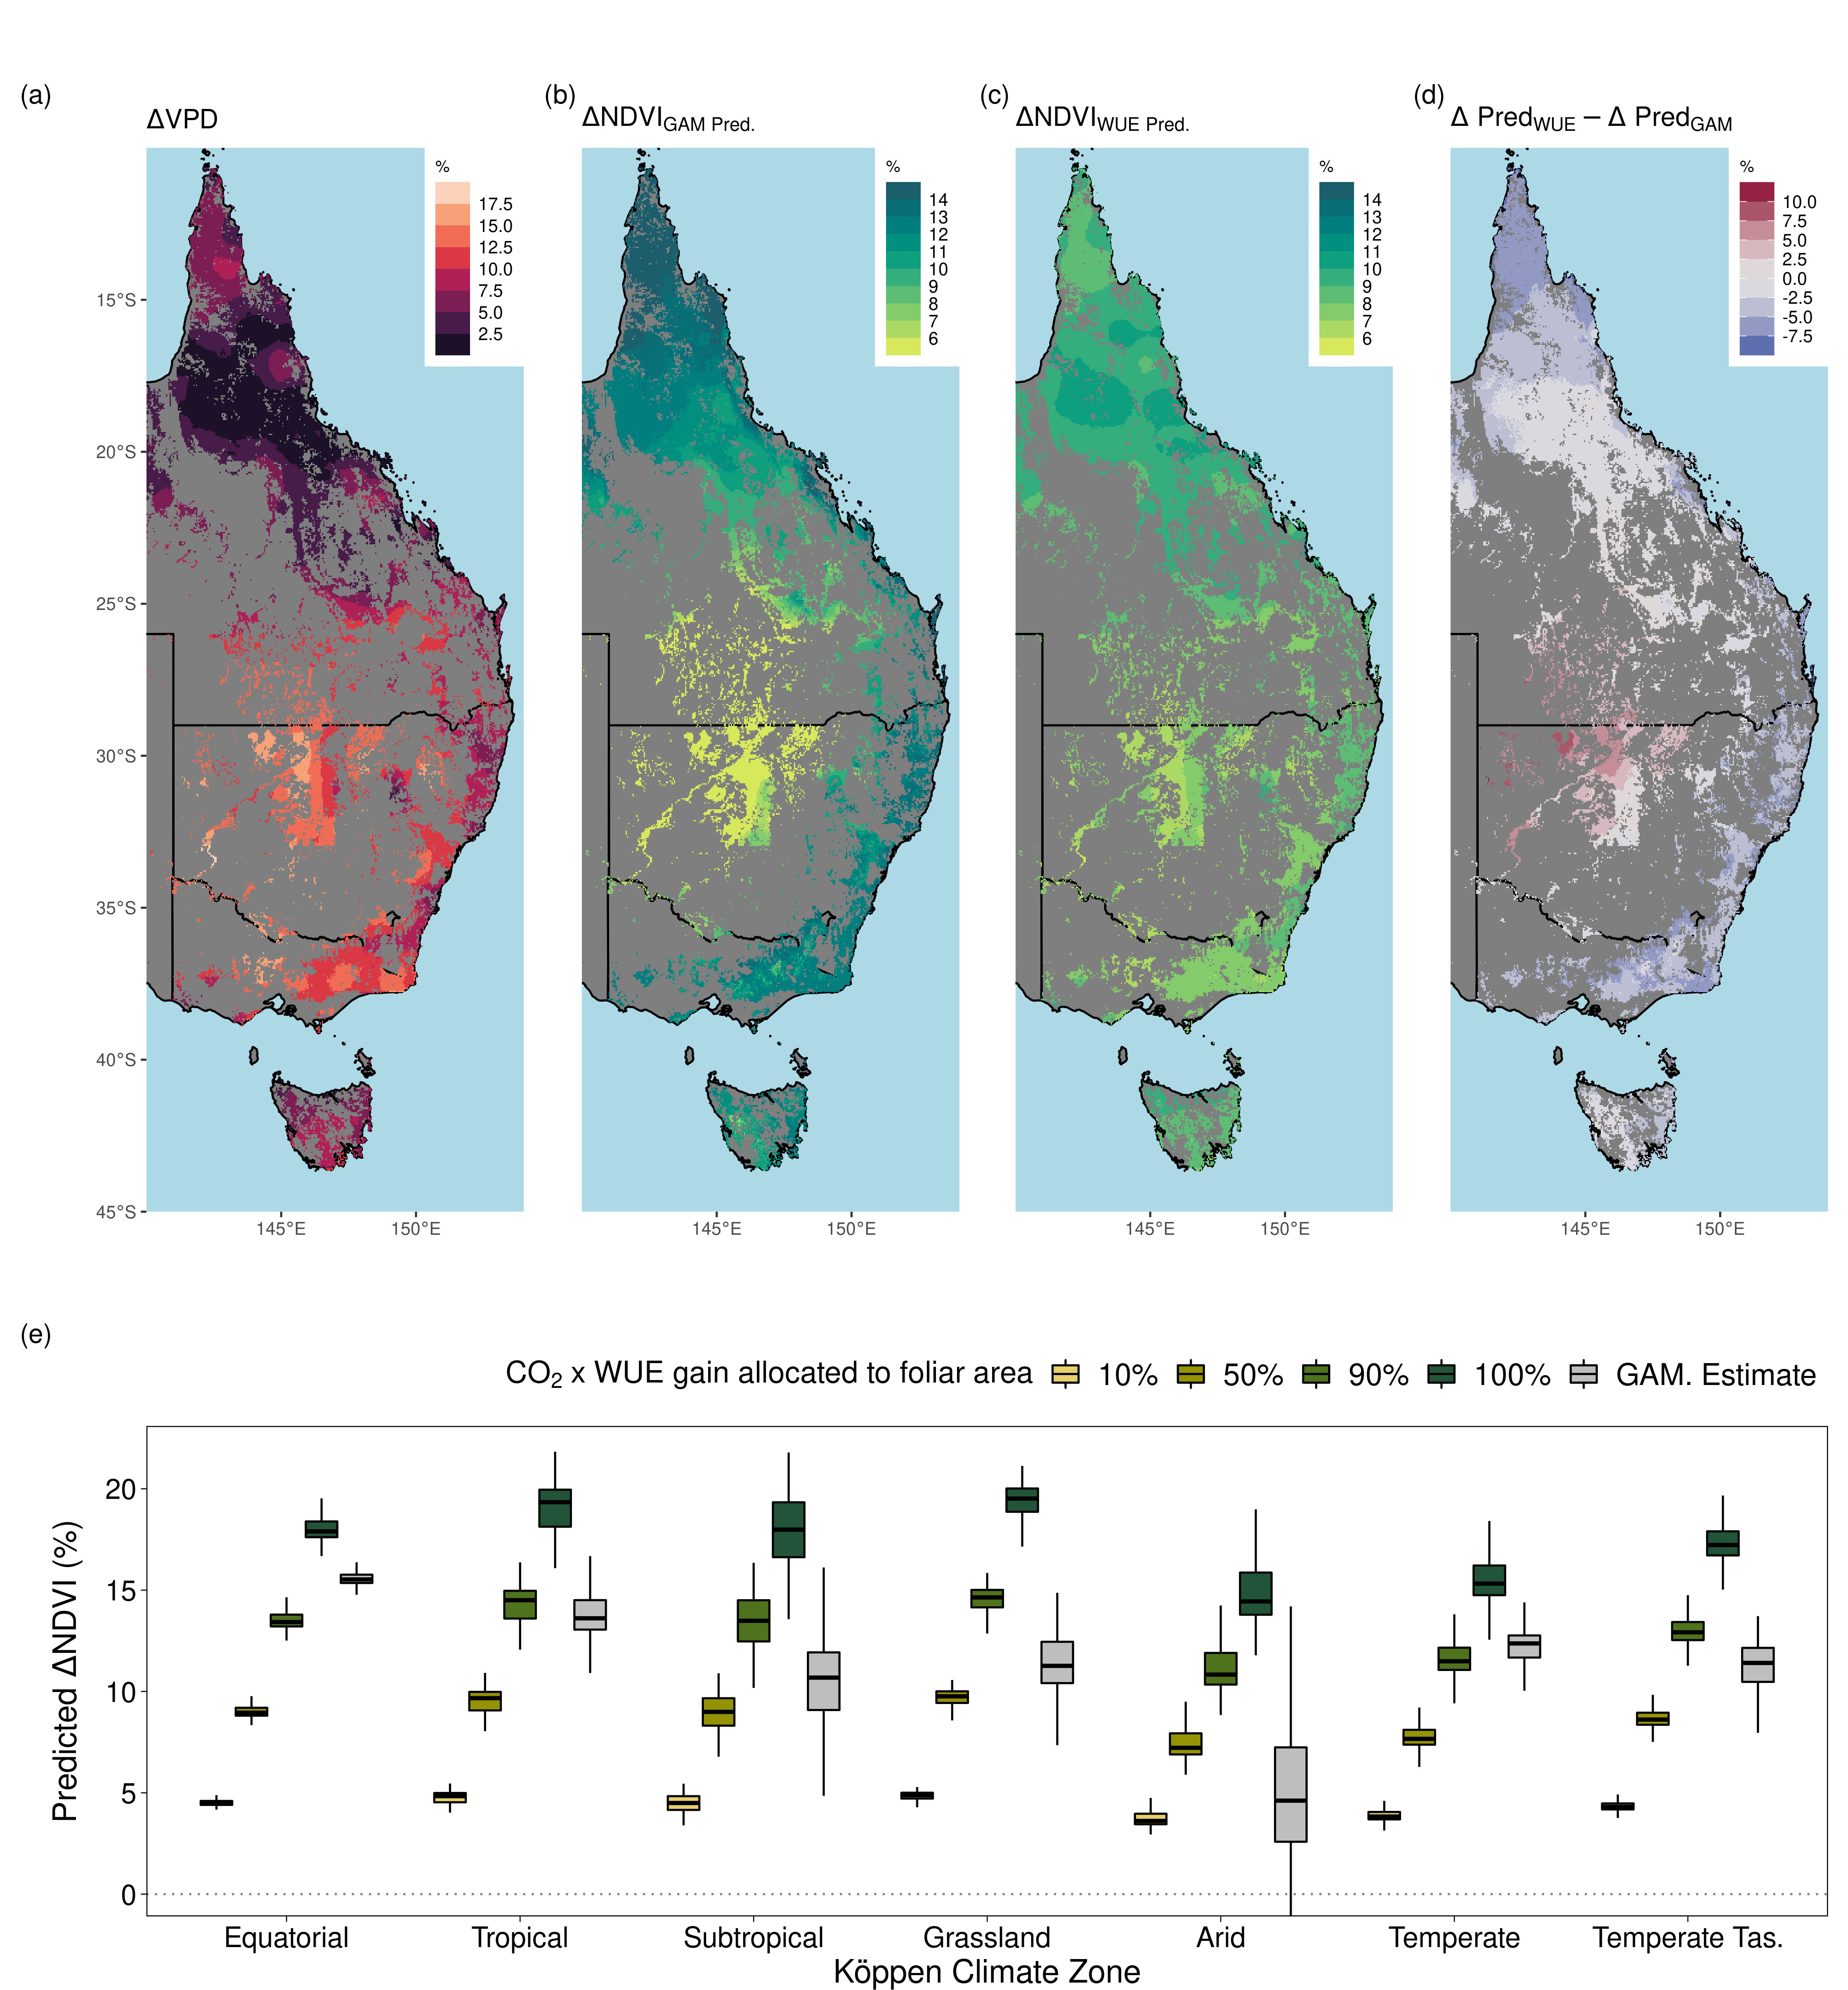
\includegraphics[width=12cm]{../../figures/Fig7_map_dVpd_gamCO2Pred_wueCO2Pred_dDifferenceBoxplot} \caption{Long-term changes in vapor pressure deficit, and comparison between the $\Delta~NDVI$ due to $CO_2$ and the expected $CO_2$ fertilization effect on foliar area due to gains in water use efficiency (WUE). (a) The relative increase in the annual mean of vapor pressure deficit (VPD) between 1982-2019. (b) The predicted relative increase in NDVI due to $CO_2$ (methods - eq 14) with a concurrent increase in VPD. (c) The relative expected increase in NDVI following the theoretical WUE prediction where 50\% of the gain is allocated to foliar area (methods - eq 11).}\label{fig:unnamed-chunk-6}
\end{figure}
\clearpage

\subsection{Co-occurring shifts in aridity, NDVI, and vegetation cover}

The shifts in P:PET and NDVI were accompanied by vegetation cover
changes in some regions. Most notably, the Arid and Temperate regions
experienced the strongest zonally averaged declines in P:PET (Fig. 8a)
and increases in VPD (Fig. S8). Seasonal greening trends were relatively
similar apart from the aforementioned exceptions in the Grassland. The
MODIS vegetation continuous fraction data from 2001-2018 indicated most
regions experienced modest changes in tree vegetation cover. The largest
decline in tree cover occurred in the Temperate regions (Fig. 8c,S10.
Most regions experienced declines in non-vegetated (bare) cover,
increases in non-tree vegetation, and modest change in tree-cover (Fig.
8c), however the proportional increase of non-tree vegetation typically
exceeded tree cover increases (Fig. S10).

\clearpage 
\begin{figure}
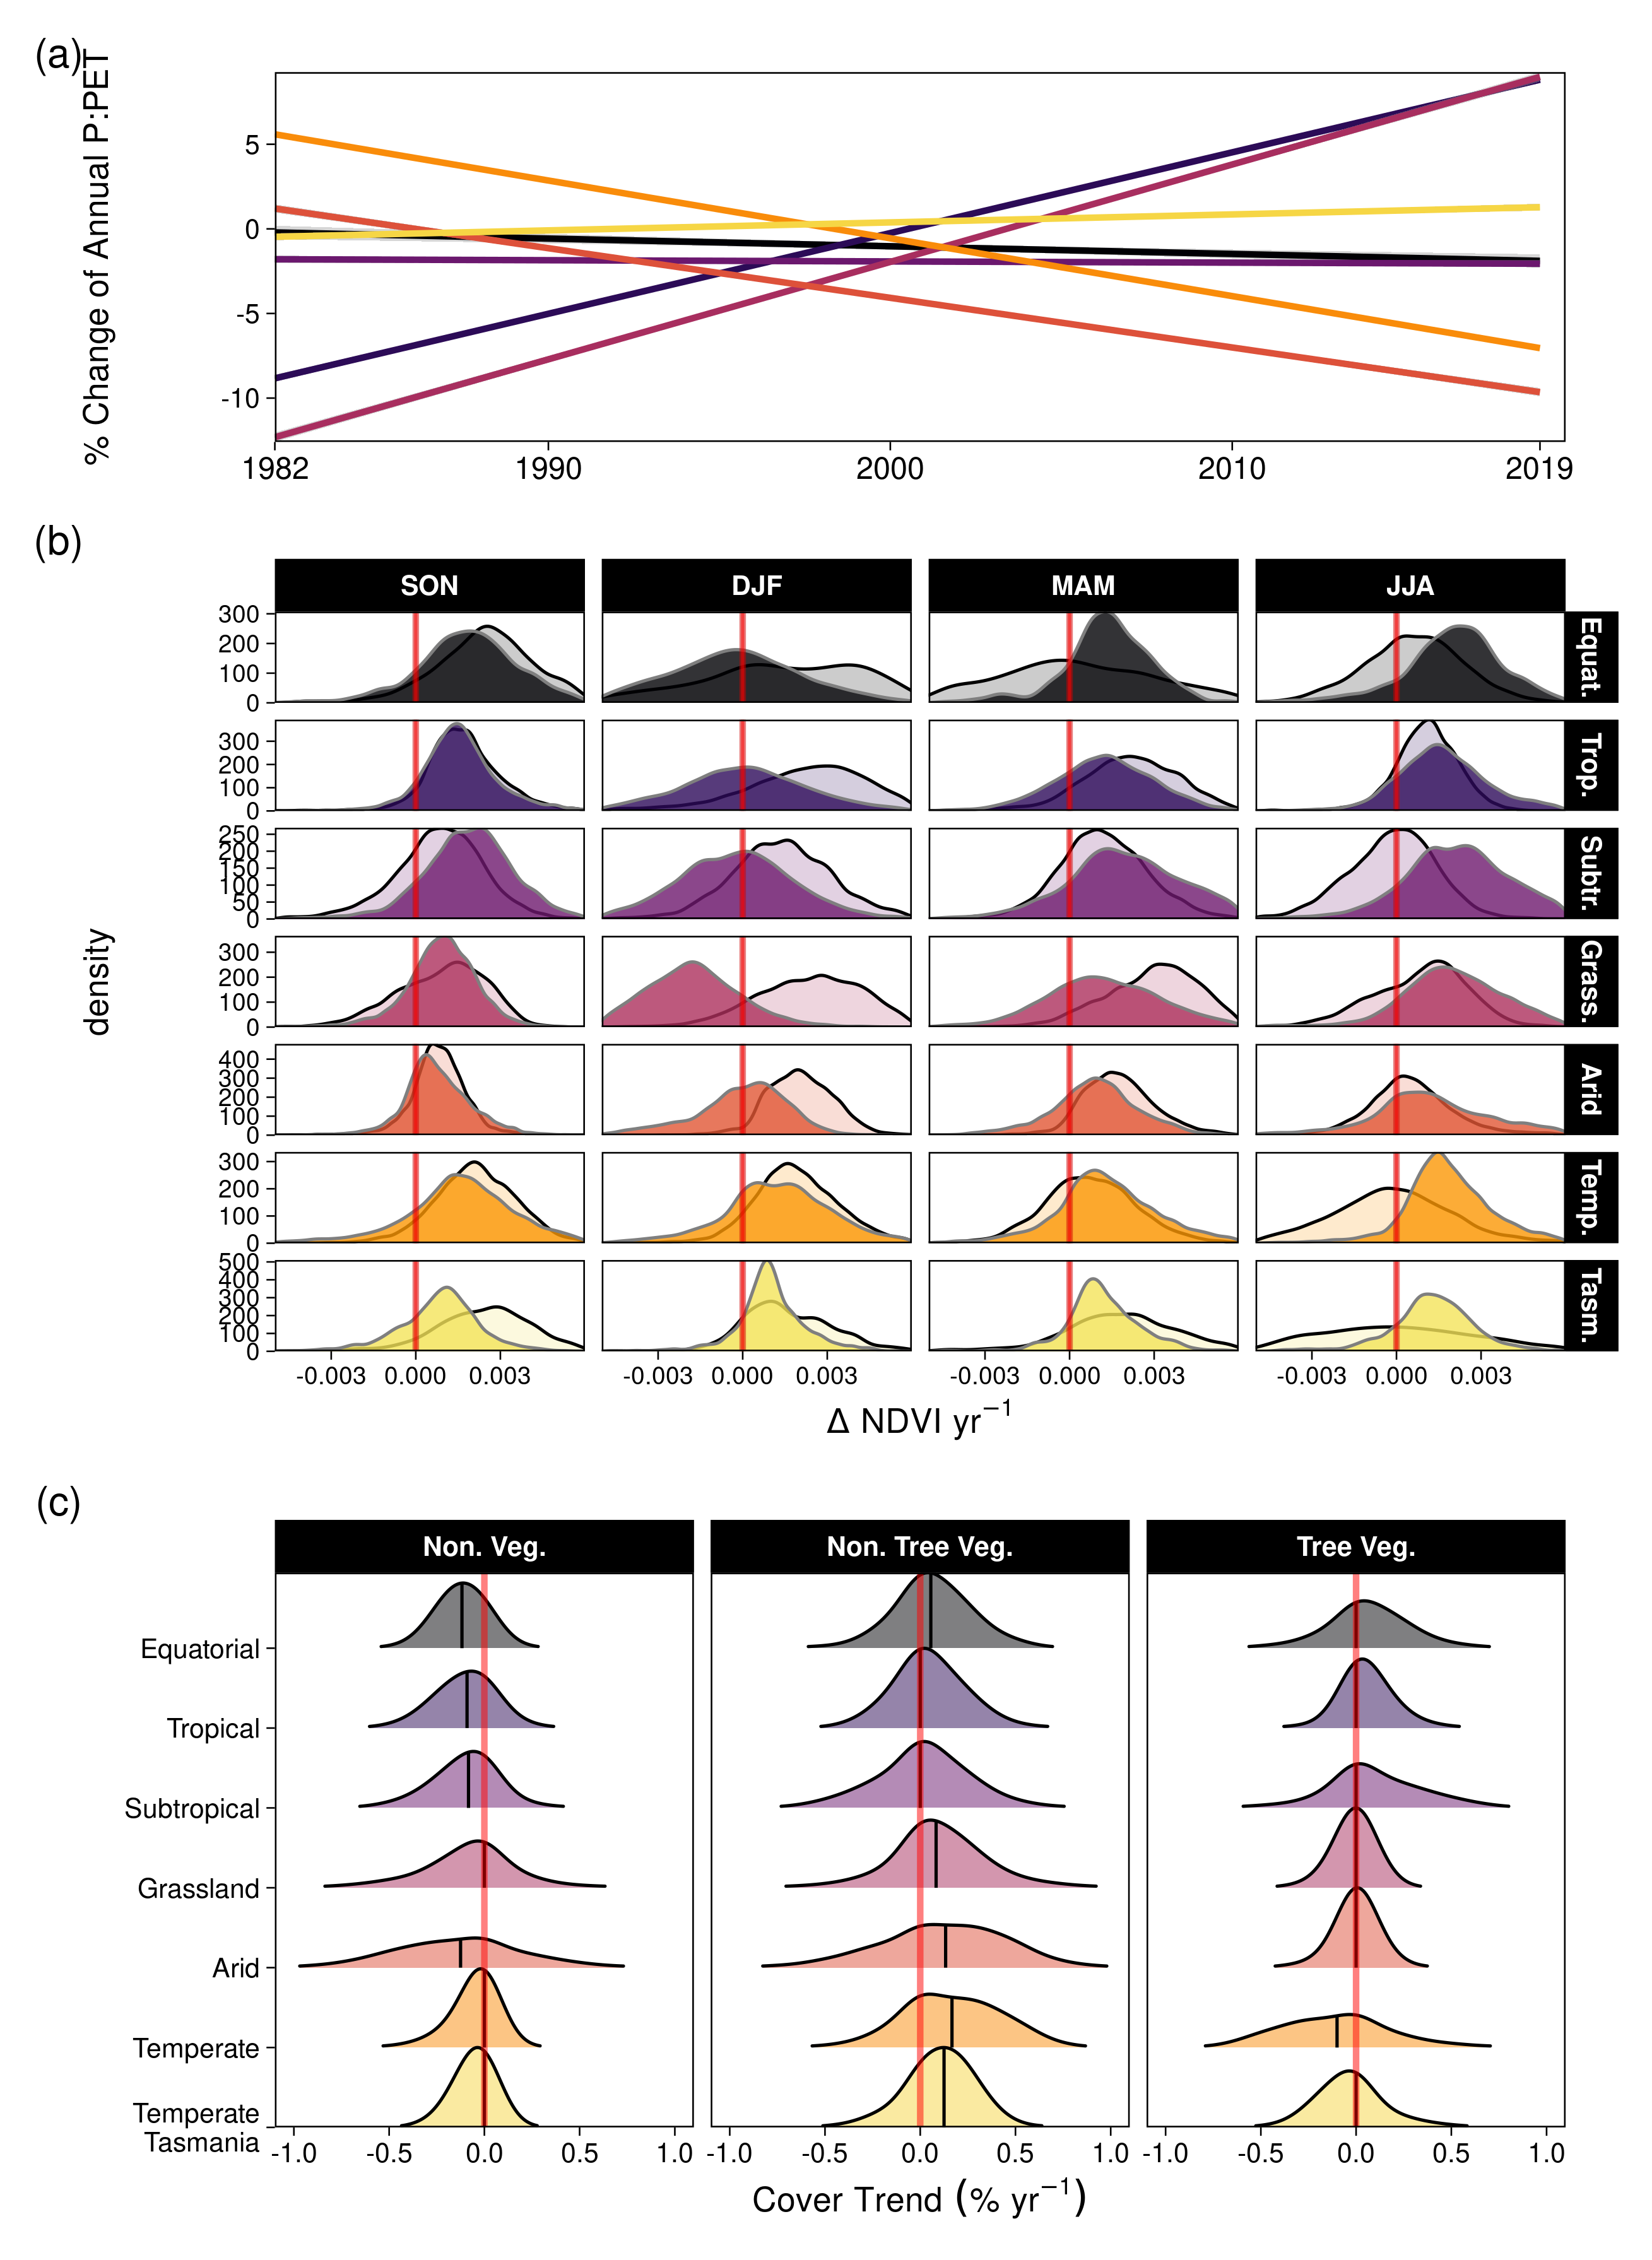
\includegraphics[width=12cm]{../../figures/Fig8_PPET_change_ThielSen_VCF} \caption{The relative percentage change in P:PET by climate zone and corresponding distributions of $\Delta~NDVI~yr^-1$ and percentage annual change in vegetation cover fraction. (a) The linear relative changes in annual P:PET trend by climate zone between 1982-2019, as estimated by robust regression (methods). (b) Distribution of linear long term NDVI trends for the six climate clusters by season using the Theil-Sen estimator. Filled distributions are trends from the MODIS sensors (2001-2019) and transparent (black outline) distributions are from the AVHRR sensors (1982-2000). (c) Distributions of the linear pixel level trends using the Theil-Sen estimator for non-vegetated cover, non-tree vegetation cover, and tree cover between 2000-2018. The 25, 50, and 75\% quantiles are overlaid. \newline Note: Climate zone abbreviations are as follows: Equatorial (Equat.), Tropical (Trop.), Subtropical (Subtr.), Grassland (Grass.), Temperate (Temp.), and Temperate Tasmania (Tasm.).}\label{fig:unnamed-chunk-7}
\end{figure}
\clearpage

\section{Discussion}

\subsection{\texorpdfstring{Australian woody vegetation as model systems
to quantify CO\textsubscript{2}
fertilization}{Australian woody vegetation as model systems to quantify CO2 fertilization}}

Australia is ideal to explore the CO\textsubscript{2} contribution
towards vegetation greening because there are fewer confounding effects
to drive greening. Forest trees are evergreen and the growing season is
rarely limited by temperature or radiation. The study region spans a
large moisture gradient (Fig. S1a), but unlike much of the global
tropics, the large majority of the study region is not so cloudy as to
prevent multiple high quality multispectral satellite retrievals per
month. Australia has also not been subjected to other prominent drivers
of greening such as nitrogen deposition
\citep{ackermanGlobalEstimatesInorganic2019}. Nevertheless, Australia
has experienced notable land-use change during the study period such as
high rates of deforestation in Queensland and northern New South Wales
\citep{evansDeforestationAustraliaDrivers2016}. However, we excluded
affected pixel locations from the analysis.

Prior global analyses on warm arid environments have quantified the
CO\textsubscript{2} effect on greening
\citep{donohueImpactCOFertilization2013b}, yet a more expansive
global-scale analysis of all terrestrial vegetation using dynamic global
vegetation model attribution did not connect Australia's greening to
changes in atmospheric CO\textsubscript{2} concentration
\citep{zhuGreeningEarthIts2016a}. Australian studies documented the
greening trend up to 2010 using the long-term AVHRR record
\citep{donohueClimaterelatedTrendsAustralian2009c, ukkolaReducedStreamflowWaterstressed2016b}
and have been able to partially attribute CO\textsubscript{2} as a
driver of greening in sub-humid and semi-arid regions. Here we advanced
upon prior research to separate the effects of disturbance, and changes
in aridity and moisture in order to quantify the CO\textsubscript{2}
fertilization effect across the full spectrum of moisture availability
experienced by Australian woody ecosystems, notably for 38 years.

\subsection{Regional differences in greening and browning through time}

Despite the region's high decadal scale variability of NDVI (Fig. 4),
the nearly four decade long record allowed us to separate the
CO\textsubscript{2} effect on NDVI from the anomalies caused by drought
(e.g.~2003-2009) or high rainfall (e.g.~La Niña 2010-2011). Although the
long-term greening trends we document in the nine years following
earlier studies are generally consistent
\citep{donohueClimaterelatedTrendsAustralian2009c, ukkolaReducedStreamflowWaterstressed2016b},
our results diverge and lead to key differences in interpretation of why
NDVI has continued to increase. First, while the relative increase in
NDVI between the 1982-2000 AVHRR epoch (5.7\%) and the 2001-2019 MODIS
epoch (5.1\%) are comparable (Figs. 3b,8b), the underlying reasons for
the change differ. VPD changed minimally between 1982-2000, whereas it
rapidly increased between 2001-2019 (SM Fig. 8). These increases were
largest in the most Arid and Temperate regions (12.7\% and 11\% since
1982, respectively; Fig. 6a), and when coupled with seasonal reductions
in precipitation (Fig. S2) these would have partially offset benefits
from increased intrinsic water-use efficiency (equation 17). In
contrast, more than half of the Equatorial, Tropical, Subtropical and
Grassland regions in northern Queensland experienced increases in
precipitation since 1982 {[}Fig. S2;
\citet{ukkolaExploringStationarityAustralian2019c}{]}, thus allowing
these locations to exceed the predicted NDVI increases from the WUE
model (Fig. 7d).

It should be noted not all regions experienced consistent greening
trends throughout the observation period. For example, `greening'
shifted to `browning' during the austral summer (Dec - Feb) in the Arid
and Grassland regions of Queensland between the 1982-2000 and 2001-2019
records (Fig. 3b). It is unclear why browning occurred during austral
summer time in the Grassland region (Figs. 3b,4,8b). The declines in
NDVI during 2001-2019 may have been meteorologically driven and related
to shifts in the distribution of wet and dry season precipitation (Fig.
S2). Alternatively, the shift could be due to changes in fire and cattle
management that have been particularly prevalent across regions of
Queensland in recent decades \citep{seabrookCattleCropsClearing2006}.
Further, greening may have been suppressed in parts of Queensland
because cattle ranching activity has intensified and has driven forest
conversion to managed pasture in the region
\citep{mcalpineIncreasingWorldConsumption2009}.

\subsection{\texorpdfstring{Attributing a CO\textsubscript{2}
fertilization contribution towards
greening}{Attributing a CO2 fertilization contribution towards greening}}

Plants increase their rates of photosynthesis in response to rising
atmospheric CO\textsubscript{2}, whilst also reducing stomatal
conductance, which reduces evaporative losses and combined, the two
responses lead to greater WUE
\citep{ainsworthResponsePhotosynthesisStomatal2007, morisonSensitivityStomataWater1985}.
In water-limited ecosystems, it has been hypothesized that this
physiological response by plants to CO\textsubscript{2} should result in
increased leaf biomass
\citep{donohueImpactCOFertilization2013b, ukkolaReducedStreamflowWaterstressed2016b}.
While all our statistical approaches indicated a year round positive
CO\textsubscript{2} effect, in contrast to theory the effect was
consistently greater in regions with higher P:PET (Figs. 5-7;S4-7). Our
analysis also diverges with a global coarse-scale analysis that found
weakening of the CO\textsubscript{2} fertilization effect across both
southeastern and northern Australia \citep{wangRecentGlobalDecline2020}.
We found no meaningful difference in the CO\textsubscript{2}
attributable effect towards greening between the AVHRR 1982-2000 and
MODIS 2001-2019 epochs to support the finding of temporally weakening
CO\textsubscript{2} effect (Fig. 6). The WUE model predicted similar
relative rates of NDVI increase between the two epochs (4.5\% and 4.7\%
for AVHRR and MODIS), yet for different reasons. CO\textsubscript{2}
increased by 30 ppm between 1982-2000 while VPD changed minimally and
precipitation increased in Queensland and the Arid region (Fig. S8); all
of which are favorable to increasing NDVI. In contrast, the larger
CO\textsubscript{2} increase between 2001-2019 (40 ppm) was offset by a
spatially ubiquitous increase of VPD (3.7\%, CI={[}-0.4\%,8.6\%{]}; Fig.
S8) and the occurrence of two multi-year droughts (Millennium Drought
2003-2009, and The Big Dry 2017-2020). Despite the widespread evidence
of the CO\textsubscript{2} effect, the WUE model notably underpredicted
greening in some regions (Fig. 7).

\subsection{Deviations from WUE}

We found the CO\textsubscript{2} effect on foliar area was the smallest
in the driest climate regions (Figs. 5-6,S4-7). This was at odds with
the WUE prediction (at 50\% allocation; Fig. 7e), and contrary to
expectation that the greatest WUE-derived benefit from
CO\textsubscript{2} would be in drier climates
{[}donohue\_etal17,mcmurtrieWhyPlantgrowthResponse2008{]}. These
deviations may have resulted from ecosystems processes beyond the scope
of a simple model, such as the phenology of the vegetation composition,
and disturbances not captured by the satellite products (e.g.~small
fires, grazing). Browning in the Grassland region (Fig. 3b,S3) may have
been caused by distinct dry season phenological differences between
overstory woody vegetation and understory C\textsubscript{4} grasses
\citep{mooreReviewsSynthesesAustralian2016}(Moore et al., 2016), which
are dominant there {[}murphySeasonalWaterAvailability2007{]}.
C\textsubscript{4} grasses may have been favored over C\textsubscript{3}
because precipitation increased during the austral summer over the
course of the study (Fig. S2) and this higher concentration of rainfall
during the warmest months is thought to favor C\textsubscript{4} grasses
\citep{hattersleyDistributionC3C41983a, knappResolvingDustBowl2020, murphySeasonalWaterAvailability2007}.
Finally, the linear dependency of leaf area upon VPD in the theoretical
model may be ill-suited for extreme anomalously arid conditions because
NDVI observations suggest a strongly nonlinear relationship with large
VPD anomalies (Fig. S11).

We explored how much of the higher WUE benefit would have to be
allocated to match the GAM estimated CO\textsubscript{2}-attributed
changes in NDVI. Allocation rates far greater than 50\% would be
required to match the WUE prediction in the Tropical and Equatorial
zones (Figure 7e), whereas allocation would need to be less than 50\% to
match the GAM estimate in the Arid region. The Arid region experienced
the greatest relative increase in VPD (Fig. 7a, S8), yet the theoretical
model still predicted a small but positive increase in NDVI (Fig. 7c)
which the GAM estimate suggests would be closer to a 10\% rather than
50\% foliar allocation level from the WUE benefit (Fig. 7d).
Nevertheless, the smaller effect over the Arid region was consistent
with earlier observational findings across Australia
\citep{ukkolaReducedStreamflowWaterstressed2016b}(Ukkola et al., 2016)
and experimentation from the Nevada Desert FACE experiment
\citep{smithLongtermResponseMojave2014}.

\subsection{\texorpdfstring{Relation to ecosystem CO\textsubscript{2}
fertilization
experiments}{Relation to ecosystem CO2 fertilization experiments}}

Notably, a four year long ecosystem-scale CO\textsubscript{2}
manipulation experiment carried out in a mature Eucalyptus woodland in
Sydney (EucFACE) did not observe an increase in leaf area under elevated
CO\textsubscript{2} \citep{jiangFateCarbonMature2020b}. The experimental
site is located upon phosphorus poor soils, typical of Australia. The
lack of a leaf area growth response observed at EucFACE is not
necessarily inconsistent with the greening effect observed in this
study. Our observational window of 38 years is much longer than the
elevated CO\textsubscript{2} exposure time in the experiment \citep[four
years in][]{jiangFateCarbonMature2020b}, covers different
CO\textsubscript{2} increments (historical vs future) and could imply
that woodlands are eventually able to liberate belowground phosphorus to
support greater biomass growth on longer timescales. Increased
autotrophic soil respiration and belowground productivity were observed
at EucFACE under elevated CO\textsubscript{2} exposure
\citep{drakeShorttermCarbonCycling2016, jiangFateCarbonMature2020b}, as
was a brief period of enhanced nitrogen and phosphorus mineralization
\citep{hasegawaElevatedCarbonDioxide2016}. Over time, this increased
investment of carbon belowground could potentially liberate sufficient
phosphorus to support an expansion of leaf area. The reduced allocation
to foliar area in the Arid region (Fig. 7e) may reflect that extra
carbon derived from CO\textsubscript{2} is allocated belowground to
increase water uptake or mitigate other resource limitations such as
soil phosphorus \citep{jiangLowPhosphorusSupply2020}.

\subsection{Vegetation composition shifts}

Most grid-cell locations in the Temperate zone experienced simultaneous
apparent declines in tree cover and increases in non-tree vegetation
cover (e.g.~grasses/shrubs) (Figs. 8c, S10). This is surprising because
we focused this regression analysis on 2001-2018 in order to exclude the
reduced tree cover due to the catastrophic megafires of 2019/20
\citep{nolanCausesConsequencesEastern2020}. Some may question the
veracity of the MODIS Vegetation Continuous Fraction product
\citep{dimiceliMOD44BMODISTerra2017} to accurately distinguish
Australian tree cover from non-tree vegetation, however this pattern is
consistent with a recent LiDAR derived tree-cover time series of
Australia \citep{liaoWoodyVegetationCover2020}. This suggests the
drought starting in 2017 was already killing trees prior to the 2019/20
megafires. Field observations of tree decline remain relatively rare,
but a citizen science initiative has documented more than 300 locations
of non-fire related mass tree mortality between 2018-2020
\citep{atlasoflivingaustraliaDeadTreeDetective}. Similarly, a study
using an experimental constrained plant hydraulics model to predict the
regions at risk of drought-induced tree mortality, found greater risk in
the same arid regions of southeast Australian forests and woodlands
\citep{dekauweIdentifyingAreasRisk2020b}. These predicted regions of
mortality coincide with where we document the greening trends that fell
short of the theoretical WUE expectation. These rapid shifts in
vegetation underlie the need for greater continuous field vegetation
monitoring to capture change imposed by climate extremes.

\conclusions[Conclusions]We separated the effects of disturbance and
meteorological anomalies with statistical models to show increasing
CO\textsubscript{2} produced nearly four decades of widespread
vegetation greening across eastern Australia. The large agreement
between a theoretical model and the statistically estimated
CO\textsubscript{2} effect indicated that greening resulted through an
increase in water use efficiency. Vegetation greening occurred despite a
highly variable and increasingly arid climate, and on soils particularly
poor in phosphorus which have likely acted as a constraint on growth.
While rising atmospheric CO\textsubscript{2} ameliorated what would have
been a browning woody ecosystem response to declining P:PET, the
CO\textsubscript{2} effect was insufficient to promote greening when
both P and P:PET experienced long-term decline, as observed in the more
arid regions in our study. Further, it is unknown whether further
increases of atmospheric CO\textsubscript{2} will continue to enable
vegetation to mitigate increases of aridity and VPD under future
warming. It is also unclear if trees or grasses are the primary
contributors to the recent greening trend. Future localised work is
urgently needed to better understand recent changes in tree and grass
competition under an increasingly arid climate, which will be essential
to help forecast ecosystem resilience. Finally, our results have
important implications for understanding Australia's terrestrial water
availability. Greening trends signal changes in evapotranspiration and
runoff, and therefore need to be considered in planning for future land
and water resource management on the world's driest inhabited continent.



\codedataavailability{All data used are publicly available from sources
listed in Table S1. Processed data used in model fitting and figures can
be accessed via Zenodo data repository: {[}future repository link{]}. A
git repository with all associated data processing, analysis, and code
to reproduce figures is located at:
https://github.com/sw-rifai/eastern-Australia-CO2-NDVI-change.} %% use this section when having data sets and software code available



%%%%%%%%%%%%%%%%%%%%%%%%%%%%%%%%%%%%%%%%%%
%% optional

%%%%%%%%%%%%%%%%%%%%%%%%%%%%%%%%%%%%%%%%%%
\appendix
\section{Figures and tables in appendices}
\subsection{Option 1}

If you sorted all figures and tables into the sections of the text,
please also sort the appendix figures and appendix tables into the
respective appendix sections. They will be correctly named
automatically.

\subsection{Option 2}

If you put all figures after the reference list, please insert appendix
tables and figures after the normal tables and figures.

\texttt{\textbackslash{}appendixfigures} needs to be added in front of
appendix figures \texttt{\textbackslash{}appendixtables} needs to be
added in front of appendix tables

Please add \texttt{\textbackslash{}clearpage} between each table and/or
figure. Further guidelines on figures and tables can be found below.
Regarding figures and tables in appendices, the following two options
are possible depending on your general handling of figures and tables in
the manuscript environment: To rename them correctly to A1, A2, etc.,
please add the following commands in front of them:
\noappendix

%%%%%%%%%%%%%%%%%%%%%%%%%%%%%%%%%%%%%%%%%%
\authorcontribution{S.W.R., M.G.D.K., P.M., L.A.C., B.E.M., and A.J.P.
designed the study. S.W.R. analyzed the data and produced the figures.
S.W.R and A.M.U. processed climate data. S.W.R. wrote the first draft
with M.G.D.K., and all authors have contributed to writing and revising
the manuscript.} %% optional section

%%%%%%%%%%%%%%%%%%%%%%%%%%%%%%%%%%%%%%%%%%
\competinginterests{The authors declare no competing
interests.} %% this section is mandatory even if you declare that no competing interests are present

%%%%%%%%%%%%%%%%%%%%%%%%%%%%%%%%%%%%%%%%%%
\disclaimer{NA.} %% optional section

%%%%%%%%%%%%%%%%%%%%%%%%%%%%%%%%%%%%%%%%%%
\begin{acknowledgements}
S.W.R., M.G.D.K., A.J.P., L.A.C, and P.M., acknowledge support from the
Australian Research Council Discovery Grant (DP190101823). S.W.R.,
M.G.D.K., A.M.U., and A.J.P. acknowledge support from the ARC Centre of
Excellence for Climate Extremes (CE170100023). M.G.D.K. was also
supported by the NSW Research Attraction and Acceleration Program and
A.M.U. by an ARC Discovery Early Career Researcher Award (DE200100086).
B.E.M. acknowledges support from ARC Laureate Fellowship FL190100003. We
are grateful to Randall J. Donohue (CSIRO Land and Water) for valuable
discussion and comments on drafts of this manuscript.
\end{acknowledgements}

%% REFERENCES
%% DN: pre-configured to BibTeX for rticles

%% The reference list is compiled as follows:
%%
%% \begin{thebibliography}{}
%%
%% \bibitem[AUTHOR(YEAR)]{LABEL1}
%% REFERENCE 1
%%
%% \bibitem[AUTHOR(YEAR)]{LABEL2}
%% REFERENCE 2
%%
%% \end{thebibliography}

%% Since the Copernicus LaTeX package includes the BibTeX style file copernicus.bst,
%% authors experienced with BibTeX only have to include the following two lines:
%%
\bibliographystyle{copernicus}
\bibliography{test.bib}
%%
%% URLs and DOIs can be entered in your BibTeX file as:
%%
%% URL = {http://www.xyz.org/~jones/idx_g.htm}
%% DOI = {10.5194/xyz}


%% LITERATURE CITATIONS
%%
%% command                        & example result
%% \citet{jones90}|               & Jones et al. (1990)
%% \citep{jones90}|               & (Jones et al., 1990)
%% \citep{jones90,jones93}|       & (Jones et al., 1990, 1993)
%% \citep[p.~32]{jones90}|        & (Jones et al., 1990, p.~32)
%% \citep[e.g.,][]{jones90}|      & (e.g., Jones et al., 1990)
%% \citep[e.g.,][p.~32]{jones90}| & (e.g., Jones et al., 1990, p.~32)
%% \citeauthor{jones90}|          & Jones et al.
%% \citeyear{jones90}|            & 1990

\end{document}
